\documentclass[twoside]{book}

% Packages required by doxygen
\usepackage{fixltx2e}
\usepackage{calc}
\usepackage{doxygen}
\usepackage[export]{adjustbox} % also loads graphicx
\usepackage{graphicx}
\usepackage[utf8]{inputenc}
\usepackage{makeidx}
\usepackage{multicol}
\usepackage{multirow}
\PassOptionsToPackage{warn}{textcomp}
\usepackage{textcomp}
\usepackage[nointegrals]{wasysym}
\usepackage[table]{xcolor}

% Font selection
\usepackage[T1]{fontenc}
\usepackage[scaled=.90]{helvet}
\usepackage{courier}
\usepackage{amssymb}
\usepackage{sectsty}
\renewcommand{\familydefault}{\sfdefault}
\allsectionsfont{%
  \fontseries{bc}\selectfont%
  \color{darkgray}%
}
\renewcommand{\DoxyLabelFont}{%
  \fontseries{bc}\selectfont%
  \color{darkgray}%
}
\newcommand{\+}{\discretionary{\mbox{\scriptsize$\hookleftarrow$}}{}{}}

% Page & text layout
\usepackage{geometry}
\geometry{%
  a4paper,%
  top=2.5cm,%
  bottom=2.5cm,%
  left=2.5cm,%
  right=2.5cm%
}
\tolerance=750
\hfuzz=15pt
\hbadness=750
\setlength{\emergencystretch}{15pt}
\setlength{\parindent}{0cm}
\setlength{\parskip}{3ex plus 2ex minus 2ex}
\makeatletter
\renewcommand{\paragraph}{%
  \@startsection{paragraph}{4}{0ex}{-1.0ex}{1.0ex}{%
    \normalfont\normalsize\bfseries\SS@parafont%
  }%
}
\renewcommand{\subparagraph}{%
  \@startsection{subparagraph}{5}{0ex}{-1.0ex}{1.0ex}{%
    \normalfont\normalsize\bfseries\SS@subparafont%
  }%
}
\makeatother

% Headers & footers
\usepackage{fancyhdr}
\pagestyle{fancyplain}
\fancyhead[LE]{\fancyplain{}{\bfseries\thepage}}
\fancyhead[CE]{\fancyplain{}{}}
\fancyhead[RE]{\fancyplain{}{\bfseries\leftmark}}
\fancyhead[LO]{\fancyplain{}{\bfseries\rightmark}}
\fancyhead[CO]{\fancyplain{}{}}
\fancyhead[RO]{\fancyplain{}{\bfseries\thepage}}
\fancyfoot[LE]{\fancyplain{}{}}
\fancyfoot[CE]{\fancyplain{}{}}
\fancyfoot[RE]{\fancyplain{}{\bfseries\scriptsize Generated by Doxygen }}
\fancyfoot[LO]{\fancyplain{}{\bfseries\scriptsize Generated by Doxygen }}
\fancyfoot[CO]{\fancyplain{}{}}
\fancyfoot[RO]{\fancyplain{}{}}
\renewcommand{\footrulewidth}{0.4pt}
\renewcommand{\chaptermark}[1]{%
  \markboth{#1}{}%
}
\renewcommand{\sectionmark}[1]{%
  \markright{\thesection\ #1}%
}

% Indices & bibliography
\usepackage{natbib}
\usepackage[titles]{tocloft}
\setcounter{tocdepth}{3}
\setcounter{secnumdepth}{5}
\makeindex

% Hyperlinks (required, but should be loaded last)
\usepackage{ifpdf}
\ifpdf
  \usepackage[pdftex,pagebackref=true]{hyperref}
\else
  \usepackage[ps2pdf,pagebackref=true]{hyperref}
\fi
\hypersetup{%
  colorlinks=true,%
  linkcolor=blue,%
  citecolor=blue,%
  unicode%
}

% Custom commands
\newcommand{\clearemptydoublepage}{%
  \newpage{\pagestyle{empty}\cleardoublepage}%
}

\usepackage{caption}
\captionsetup{labelsep=space,justification=centering,font={bf},singlelinecheck=off,skip=4pt,position=top}

%===== C O N T E N T S =====

\begin{document}

% Titlepage & ToC
\pagenumbering{alph}
\begin{titlepage}
\vspace*{7cm}
\begin{center}%
{\Large segmentation }\\
\vspace*{1cm}
{\large Generated by Doxygen 1.8.13}\\
\end{center}
\end{titlepage}
\clearemptydoublepage
\pagenumbering{roman}
\tableofcontents
\clearemptydoublepage
\pagenumbering{arabic}

%--- Begin generated contents ---
\chapter{disp\+Blobber}
\label{md_C_1_dev_icub-contrib-iit_segmentation_dispBlobber_README}
Module to detect the closest proto-\/object in the robot\textquotesingle{}s visual field using stereo-\/vision.

\subsection*{Description}

This module takes as input a disparity map (grayscale image) and provides as output the closest (brightest) blob, which is generally an object or proto-\/object in the scene. The output is provided in the following forms\+:


\begin{DoxyItemize}
\item binary image with the segmented blob
\item cropped rectangular region enclosing the segmented blob on the input disparity map
\item 2D top-\/left (TL) and bottom-\/right (BR) pixel coordinates of the cropped rectangular region on the input disparity map -\/eventually averaged over a frame buffer of arbitrary size-\/
\item 2D pixel coordinates of the centroid of the segmented blob -\/eventually averaged over the same frame buffer-\/ on the input disparity map
\end{DoxyItemize}

If the input disparity map comes from the \href{https://github.com/robotology/stereo-vision}{\tt S\+FM} module and this module is connected to the R\+PC port of the \href{https://github.com/robotology/stereo-vision}{\tt S\+FM}, then the stereo pairs (correspondent 2D points on the other camera) and the 3D re-\/projections in the world reference frame of the above points (blob\textquotesingle{}s TL and BR R\+OI vertices and centroid) are also provided as output.

The centroid\textquotesingle{}s coordinates of the closest blob in the scene provided by this module can be fed to the \href{http://wiki.icub.org/iCub_documentation/group__actionsRenderingEngine.html}{\tt A\+RE} or directly to the \href{http://wiki.icub.org/iCub_documentation/group__iKinGazeCtrl.html}{\tt i\+Kin\+Gaze\+Ctrl} module in order to focus the robot\textquotesingle{}s gaze on the object of interest. If the data connection is streamlined then the robot keeps on focusing on the closest proto-\/object in its visual field.

Example applications of the usage of this module can be found here\+:
\begin{DoxyItemize}
\item \href{https://github.com/robotology/onthefly-recognition}{\tt onthefly-\/recognition}\+: demo to teach the i\+Cub to recognize new objects on-\/the-\/fly.
\item \href{https://github.com/GiuliaP/icubworld}{\tt icubworld}\+: application to acquire a dataset of images from the i\+Cub\textquotesingle{}s cameras while the robot is observing a set of objects shown by a human operator. The dataset can be used, e.\+g., to train/benchmark offline a visual recognition system. 
\end{DoxyItemize}
\chapter{seg2cloud}
\label{md_C_1_dev_icub-contrib-iit_segmentation_seg2cloud_README}
Module to capture pointclouds from segmented regions in 2D or 2.\+5D (depth) images

\subsection*{Description}

This module combines disparity and segmentation information in order to retrieve 3D clouds of desired 2D regions. These regions can be chosen from a user defined polygon, from a segmentation algorithm, or from 2D (in color) or 3D (in depth) flood filling. When using segmentation modules (2D or 3D), seeding can be performed automatically.

\subsection*{Dependencies}


\begin{DoxyItemize}
\item \href{https://github.com/robotology/yarp}{\tt Y\+A\+RP}
\item \href{https://github.com/robotology/icub-main}{\tt i\+Cub}
\item \href{https://github.com/robotology/icub-contrib-common}{\tt icub-\/contrib-\/common}
\item \href{http://opencv.org/}{\tt Open\+CV}
\item \href{https://github.com/robotology/stereo-vision}{\tt S\+FM}
\end{DoxyItemize}

\subsection*{Reconstruction Options}

This modules interfaces between segmentation modules and S\+FM in order to provide the 3D reconstruction of an object delimited by a contour in the image. In order to obtain this contour, 4 modes are provided\+:


\begin{DoxyItemize}
\item {\bfseries seg\+:} 2D segmentation (requires external segmentation module). When this option is called, the contour is provided by an external segmentation module.
\item {\bfseries flood\+:} 2D color flood. The object\textquotesingle{}s contour is obtained by performing a 2D color flood, based on the thresholding parameter {\itshape color\+\_\+distance}.
\item {\bfseries flood3D} 3D depth flood. The contour is determined by a flood operation performed on the depth image, controlled by the thresholding parameter {\itshape space\+\_\+distance}.
\item {\bfseries polygon} User selected polygon contour. The contour is provided by the user as a contour by selecting the vertices on a connected yarpview window.
\end{DoxyItemize}

\subsection*{Seed feeding options}

In order to select which of the possible regions of the image is segmented, a seed usually needs to be provided. In this module, the seed can be provided in several different ways\+:
\begin{DoxyItemize}
\item In the three first options above ({\ttfamily seg}, {\ttfamily flood} and {\ttfamily flood3d}) the initial seed to perform segmentation can be provided in 3 different ways\+:
\item If parameter {\ttfamily seed\+Auto} is set to {\itshape true}, the seed will be obtained automatically.
\begin{DoxyItemize}
\item In segmentations options {\ttfamily seg} and {\ttfamily flood}, seed has to be provided by a tracker whose ooutput (u v coordinates) is connected to the {\ttfamily /seg2cloud/seed\+:i} port.
\item If the segmentation option is {\ttfamily flood3d}, the seed is computed automatically as the center of the closest blob (as in the disb\+Blobber module).
\end{DoxyItemize}
\item If parameter {\ttfamily seed\+Auto} is set to {\itshape false}, the seed can be coveyed in 2 further ways\+:
\begin{DoxyItemize}
\item By clicking on a connected yarpview window whose output is connected to the {\ttfamily /seg2cloud/seed\+:i}port.
\item As {\itshape explicit u v coordinates} given after the segmentation command. For example {\ttfamily  seg 102 175 }.
\end{DoxyItemize}
\item In the case where the segmentation option is set to {\ttfamily polygon}, no seed is needed, as the region is fully provided by the user.
\end{DoxyItemize}

The results obtained with each of these options can be observed below.

\subsection*{Images of reconstruction results\+:}

\subsubsection*{seg (2D segmentation provided by \href{https://github.com/robotology/segmentation/tree/master/lbpExtract}{\tt lbp\+Exptract})}



\subsubsection*{flood (2D color flood)}



\subsubsection*{flood3D (3D spatial flood)}



\subsubsection*{polygon (Selected polygon segmentation)}



\subsection*{Documentation}

Online documentation is available here\+: \href{http://robotology.github.com/segmentation-to-pointcloud}{\tt http\+://robotology.\+github.\+com/segmentation-\/to-\/pointcloud}.

\subsection*{License}

Material included here is Copyright of {\itshape i\+Cub Facility -\/ Istituto Italiano di Tecnologia} and is released under the terms of the G\+PL v2.\+0 or later. See the file L\+I\+C\+E\+N\+SE for details. 
\chapter{Module Index}
\section{Modules}
Here is a list of all modules\+:\begin{DoxyCompactList}
\item \contentsline{section}{edison\+Segmentation}{\pageref{group__icub__edisonSegmentation}}{}
\item \contentsline{section}{graphbased\+Segmentation}{\pageref{group__icub__graphbasedSegmentation}}{}
\item \contentsline{section}{Blob Extractor}{\pageref{group__icub__blobExtractor}}{}
\item \contentsline{section}{disp\+Blobber}{\pageref{group__dispBlobber}}{}
\item \contentsline{section}{lbp\+Extract}{\pageref{group__lbpExtract}}{}
\item \contentsline{section}{seg2cloud}{\pageref{group__seg2cloud}}{}
\end{DoxyCompactList}

\chapter{Namespace Index}
\section{Namespace List}
Here is a list of all documented namespaces with brief descriptions\+:\begin{DoxyCompactList}
\item\contentsline{section}{\hyperlink{namespacelbp}{lbp} \\*Original code by philipp $<$bytefish\mbox{[}at\mbox{]}gmx\mbox{[}dot\mbox{]}de$>$ }{\pageref{namespacelbp}}{}
\end{DoxyCompactList}

\chapter{Hierarchical Index}
\section{Class Hierarchy}
This inheritance list is sorted roughly, but not completely, alphabetically\+:\begin{DoxyCompactList}
\item \contentsline{section}{Edison\+Segm\+Module}{\pageref{classEdisonSegmModule}}{}
\item \contentsline{section}{lbp\+Extract\+\_\+\+I\+D\+L\+Server}{\pageref{classlbpExtract__IDLServer}}{}
\item \contentsline{section}{yarp\+:\+:sig\+:\+:Pixel}{\pageref{classyarp_1_1sig_1_1Pixel}}{}
\item \contentsline{section}{yarp\+:\+:sig\+:\+:Segmentation\+Module\+Interface}{\pageref{classyarp_1_1sig_1_1SegmentationModuleInterface}}{}
\begin{DoxyCompactList}
\item \contentsline{section}{G\+B\+Segm\+Module}{\pageref{classGBSegmModule}}{}
\end{DoxyCompactList}
\end{DoxyCompactList}

\chapter{Data Structure Index}
\section{Data Structures}
Here are the data structures with brief descriptions\+:\begin{DoxyCompactList}
\item\contentsline{section}{\hyperlink{classEdisonSegmModule}{Edison\+Segm\+Module} \\*Edison Segmentation Module }{\pageref{classEdisonSegmModule}}{}
\item\contentsline{section}{\hyperlink{classGBSegmModule}{G\+B\+Segm\+Module} \\*Segmentation Module }{\pageref{classGBSegmModule}}{}
\item\contentsline{section}{\hyperlink{classlbpExtract__IDLServer}{lbp\+Extract\+\_\+\+I\+D\+L\+Server} \\*Lbp\+Extract\+\_\+\+I\+D\+L\+Server Interface }{\pageref{classlbpExtract__IDLServer}}{}
\item\contentsline{section}{\hyperlink{classyarp_1_1sig_1_1Pixel}{yarp\+::sig\+::\+Pixel} \\*\hyperlink{classyarp_1_1sig_1_1Pixel}{Pixel} position in the image frame }{\pageref{classyarp_1_1sig_1_1Pixel}}{}
\item\contentsline{section}{\hyperlink{classyarp_1_1sig_1_1SegmentationModuleInterface}{yarp\+::sig\+::\+Segmentation\+Module\+Interface} \\*Interface for module that performs graph-\/based segmentation }{\pageref{classyarp_1_1sig_1_1SegmentationModuleInterface}}{}
\end{DoxyCompactList}

\chapter{Module Documentation}
\section{edison\+Segmentation}
\label{group__icub__edisonSegmentation}\index{edison\+Segmentation@{edison\+Segmentation}}


Wrapper to the The E\+D\+I\+S\+ON system\+: a low-\/level vision tool that performs confidence based edge detection and synergistic image segmentation.  


Wrapper to the The E\+D\+I\+S\+ON system\+: a low-\/level vision tool that performs confidence based edge detection and synergistic image segmentation. 

\hypertarget{group__seg2cloud_intro_sec}{}\subsection{Description}\label{group__seg2cloud_intro_sec}
This module wraps around some functions of the E\+D\+I\+S\+ON system from the robust image understanding laboratory at Rutgers University.

The purpose of the module is to obtain good segmentation of color images. The image is split into regions corresponding to uniformly colored patches.

Details on the employed algorithms is provided in the following paper\+: \mbox{[}1\mbox{]} D. Comaniciu, P. Meer\+: \char`\"{}\+Mean shift\+: A robust approach toward feature space analysis\char`\"{}. I\+E\+EE Trans. Pattern Anal. Machine Intell., May 2002.

\mbox{[}2\mbox{]} P. Meer, B. Georgescu\+: \char`\"{}\+Edge detection with embedded confidence\char`\"{}. I\+E\+EE Trans. Pattern Anal. Machine Intell., 28, 2001.

\mbox{[}3\mbox{]} C. Christoudias, B. Georgescu, P. Meer\+: \char`\"{}\+Synergism in low level vision\char`\"{}. 16th International Conference of Pattern Recognition, Track 1 -\/ Computer Vision and Robotics, Quebec City, Canada, August 2001.

The edison source files are provided as a library in the edisonlib folder.

Some changes to these files had to be made in order to obtain the desired functionality. These include changes in function Get\+Regions in \hyperlink{msImageProcessor_8cpp_source}{ms\+Image\+Processor.\+cpp}\hypertarget{group__icub__blobExtractor_lib_sec}{}\subsection{Libraries}\label{group__icub__blobExtractor_lib_sec}
Y\+A\+RP library Open\+CV library\hypertarget{group__seg2cloud_parameters_sec}{}\subsection{Parameters}\label{group__seg2cloud_parameters_sec}
width, height -\/ Dimension of the images to be processed. This may differ from the dimension of the input images. Forcing a smaller dimension will save computation power at the cost of resolution. Values larger that the input image dimension will be discarded. These parameters do no influence the dimension of the output. This is always the same as the input dimension. Default\+: the size of the original image.

sigmaS -\/ The spatial bandwidth (neighborhood in the pixel domain). Default\+: 7

sigmaR -\/ The color bandwidth (neighborhood in the color color domain). Default\+: 6.\+5

minregion -\/ The minimal area for segmented regions (in pixels) Default\+: 20.\+0

grad\+Win\+Rad -\/ The radius of the window used for the computation of the gradient and confidence map (positive integer). Default\+: 2.\+0

threshold -\/ edge strength threshold (must be in the interval \mbox{[}0,1\mbox{]}) Default\+: 0.\+3

mixture -\/ mixture parameter (must be in the interval \mbox{[}0,1\mbox{]}) Default\+: 0.\+2

speedup -\/ accelerate computation by doing some approximations. Possible values 0 (N\+O\+\_\+\+S\+P\+E\+E\+D\+UP), 1 (M\+E\+D\+\_\+\+S\+P\+E\+E\+D\+UP), 2 (H\+I\+G\+H\+\_\+\+S\+P\+E\+E\+D\+UP) Default\+: M\+E\+D\+\_\+\+S\+P\+E\+E\+D\+UP

The best results have been obtained with M\+E\+D\+\_\+\+S\+P\+E\+E\+D\+UP\hypertarget{group__icub__graphbasedSegmentation_portsa_sec}{}\subsection{Ports Accessed}\label{group__icub__graphbasedSegmentation_portsa_sec}
Port with raw R\+GB image.\hypertarget{group__icub__blobExtractor_portsc_sec}{}\subsection{Ports Created}\label{group__icub__blobExtractor_portsc_sec}
/conf for module configuration, according to E\+D\+I\+S\+O\+Nsegmentation.\+thrift definition file

/raw\+Img\+:i receive the original R\+GB image to segment

/raw\+Img\+:o output the original R\+GB image

/labeled\+Img\+:o segmented image with the labels (Pixel\+Int)

/view\+Img\+:o segmented image with the colors models for each region (good to visualize)\hypertarget{group__icub__graphbasedSegmentation_in_files_sec}{}\subsection{Input Data Files}\label{group__icub__graphbasedSegmentation_in_files_sec}
None\hypertarget{group__icub__graphbasedSegmentation_out_data_sec}{}\subsection{Output Data Files}\label{group__icub__graphbasedSegmentation_out_data_sec}
None\hypertarget{group__icub__graphbasedSegmentation_conf_file_sec}{}\subsection{Configuration Files}\label{group__icub__graphbasedSegmentation_conf_file_sec}
Parameters can be put in a configuration file. Default configuration file name is edison\+Config.\+ini An example configuration file is provided in the source folder (config\+File.\+ini), containing the following\+: 
\begin{DoxyCode}
height 120
width 160
dim 3
sigmaS 10       
sigmaR 18       
minRegion 50  
gradWindRad  2 
threshold  1 
mixture  1  
speedup 1
\end{DoxyCode}
\hypertarget{group__icub__blobExtractor_tested_os_sec}{}\subsection{Tested OS}\label{group__icub__blobExtractor_tested_os_sec}
Linux and Windows.\hypertarget{group__icub__graphbasedSegmentation_example_sec}{}\subsection{Example Instantiation of the Module}\label{group__icub__graphbasedSegmentation_example_sec}

\begin{DoxyCode}
yarp server
edisonSegmentation.exe --from configFile.ini
yarpdev --device opencv\_grabber --movie H:\(\backslash\)DataSets\(\backslash\)testImages2009\_07\_21\(\backslash\)segm\_test\_icub.avi --loop --
      framerate 0.1
yarpview /raw
yarpview /view
yarp connect /grabber /edisonSegm/rawImg:i
yarp connect /edisonSegm/rawImg:o /raw
yarp connect /edisonSegm/viewImg:o /view
\end{DoxyCode}


\begin{DoxyAuthor}{Author}
Alexandre Bernardino, Elena Ceseracciu (improved module version)
\end{DoxyAuthor}
Copyright (C) 2008 Robot\+Cub Consortium

Copy\+Policy\+: Released under the terms of the G\+NU G\+PL v2.\+0.

This file can be edited at src/edison\+Segmentation/main.\+cpp. 
\section{graphbased\+Segmentation}
\label{group__icub__graphbasedSegmentation}\index{graphbased\+Segmentation@{graphbased\+Segmentation}}


Wrapper module that performs graph-\/based image segmentation exploiting the algorithm developed by Felzenszwalb and Huttenlocher (Brown University).  


Wrapper module that performs graph-\/based image segmentation exploiting the algorithm developed by Felzenszwalb and Huttenlocher (Brown University). 

\hypertarget{group__seg2cloud_intro_sec}{}\subsection{Description}\label{group__seg2cloud_intro_sec}
Wrapper module that performs graph-\/based image segmentation exploiting the algorithm developed by Felzenszwalb and Huttenlocher (Brown University). The algorithm is described in the paper \char`\"{}\+Efficient Graph-\/\+Based Image Segmentation\char`\"{}, Pedro F. Felzenszwalb and Daniel P. Huttenlocher, International Journal of Computer Vision, Volume 59, Number 2, September 2004. The original code is available from \href{http://www.cs.brown.edu/~pff/segment/}{\tt http\+://www.\+cs.\+brown.\+edu/$\sim$pff/segment/} and has been copied into the src/segmentation/graph\+Based/segment folder.\hypertarget{group__icub__blobExtractor_lib_sec}{}\subsection{Libraries}\label{group__icub__blobExtractor_lib_sec}
Y\+A\+RP library.\hypertarget{group__seg2cloud_parameters_sec}{}\subsection{Parameters}\label{group__seg2cloud_parameters_sec}

\begin{DoxyItemize}
\item {\ttfamily name} name of the module (for opened ports)
\item {\ttfamily sigma} smoothing parameter (standard deviation of a Gaussian filter used to pre-\/process image, in order to compensate for digitization artifacts)
\item {\ttfamily k} scale factor for boundary-\/detection threshold function (a larger k causes a preference for larger components).
\item {\ttfamily min\+Region} minumum size of a component.
\end{DoxyItemize}\hypertarget{group__icub__graphbasedSegmentation_portsa_sec}{}\subsection{Ports Accessed}\label{group__icub__graphbasedSegmentation_portsa_sec}
None.\hypertarget{group__icub__blobExtractor_portsc_sec}{}\subsection{Ports Created}\label{group__icub__blobExtractor_portsc_sec}

\begin{DoxyItemize}
\item /$<$module\+\_\+name$>$/raw\+Img\+:i input port where original images must be sent (default\+: G\+B\+Seg)
\item /$<$module\+\_\+name$>$/view\+Img\+:o
\item /$<$module\+\_\+name$>$/conf rpc port, accepts the commands defined in \hyperlink{}{graph\+Based\+Segmentation\+Interface.\+thrift } and documented \hyperlink{}{here }
\end{DoxyItemize}\hypertarget{group__icub__graphbasedSegmentation_in_files_sec}{}\subsection{Input Data Files}\label{group__icub__graphbasedSegmentation_in_files_sec}
None\hypertarget{group__icub__graphbasedSegmentation_out_data_sec}{}\subsection{Output Data Files}\label{group__icub__graphbasedSegmentation_out_data_sec}
None\hypertarget{group__icub__graphbasedSegmentation_conf_file_sec}{}\subsection{Configuration Files}\label{group__icub__graphbasedSegmentation_conf_file_sec}
No configuration file is needed. Parameters described in \hyperlink{group__seg2cloud_parameters_sec}{Parameters} can be provided in a configuration file; default filename is\hypertarget{group__icub__blobExtractor_tested_os_sec}{}\subsection{Tested OS}\label{group__icub__blobExtractor_tested_os_sec}
Linux and Windows.\hypertarget{group__icub__graphbasedSegmentation_example_sec}{}\subsection{Example Instantiation of the Module}\label{group__icub__graphbasedSegmentation_example_sec}
Examples of module use are provided in the app/scripts folder, and installed into app/graph\+Based\+Segm/scripts.

\begin{DoxyAuthor}{Author}
Elena Ceseracciu
\end{DoxyAuthor}
Copyright (C) 2012 R\+B\+CS -\/ Istituto Italiano di Tecnologia

Copy\+Policy\+: Released under the terms of the G\+NU G\+PL v2.\+0 and later.

This file can be edited at src/segmentation/graph\+Based/main.\+cpp. 
\section{Blob Extractor}
\label{group__icub__blobExtractor}\index{Blob Extractor@{Blob Extractor}}


Module that uses the data from the luma\+Chroma module to extract blobs that are available.  


Module that uses the data from the luma\+Chroma module to extract blobs that are available. 

\hyperlink{group__icub__blobExtractor}{Blob Extractor} application.\hypertarget{group__seg2cloud_intro_sec}{}\subsection{Description}\label{group__seg2cloud_intro_sec}
This module is responsible for extracting all the blobs based upon the icub\+\_\+luma\+Chroma module. To this end, it receives an image input from the luma\+Chroma and acts upon it to retreive the blobs and their moments (orientation and principal axes)

The commands sent as bottles to the module port /$<$mod\+Name$>$/rpc are the following\+:

(notation\+: \mbox{[}.\mbox{]} identifies a vocab, $<$.$>$ specifies a double, \char`\"{}.\char`\"{} specifies a string)

{\bfseries T\+H\+R\+E\+SH} ~\newline
format\+: \mbox{[}thresh\mbox{]} $<$10.\+0$>$ ~\newline
action\+: Applies a fixed-\/level threshold to each array element, defaults 10.\+0 (input array is the image). reply\+: ok

{\bfseries E\+R\+O\+DE} ~\newline
format\+: \mbox{[}erode\mbox{]} $<$8.\+0$>$ ~\newline
action\+: Erodes an image by using a specific structuring element, defaults 8.\+0. reply\+: ok

{\bfseries D\+I\+L\+A\+TE} ~\newline
format\+: \mbox{[}dilate\mbox{]} $<$3.\+0$>$ ~\newline
action\+: Dilates an image by using a specific structuring element., defaults 3.\+0. reply\+: ok\hypertarget{group__icub__blobExtractor_lib_sec}{}\subsection{Libraries}\label{group__icub__blobExtractor_lib_sec}

\begin{DoxyItemize}
\item Y\+A\+RP libraries, Open\+CV.
\end{DoxyItemize}\hypertarget{group__icub__blobExtractor_portsc_sec}{}\subsection{Ports Created}\label{group__icub__blobExtractor_portsc_sec}

\begin{DoxyItemize}
\item {\itshape /} $<$mod\+Name$>$/img\+:i receives the image acquired from the luma\+Chroma module previously specified through the command-\/line parameters.
\item {\itshape /} $<$mod\+Name$>$/img\+:o streams out the binary images displaying all blobs.
\item {\itshape /} $<$mod\+Name$>$/prop\+Img\+:o streams out the camera image propagated for synchronisation.
\item {\itshape /} $<$mod\+Name$>$/blobs\+:o streams out a yarp list containing all the blobs information, such as bounding box and moments if selected.
\item {\itshape /} $<$mod\+Name$>$/binary\+:o streams out a cleaned binary image containing only blobs detected (without noise).
\end{DoxyItemize}\hypertarget{group__seg2cloud_parameters_sec}{}\subsection{Parameters}\label{group__seg2cloud_parameters_sec}
--name {\itshape name} 
\begin{DoxyItemize}
\item specify the module stem-\/name, which is {\itshape blob\+Extractor} by default. The stem-\/name is used as prefix for all open ports.
\end{DoxyItemize}

--thresh {\itshape value} 
\begin{DoxyItemize}
\item specify the threshold value. Applies a fixed-\/level threshold to each array element. The default value is 10.\+0.
\end{DoxyItemize}

--erode\+\_\+itr {\itshape value} 
\begin{DoxyItemize}
\item specify the erode value. Erodes an image by using a specific structuring element. The default value is 8.\+0.
\end{DoxyItemize}

--dilate\+\_\+itr {\itshape value} 
\begin{DoxyItemize}
\item specify the dilate value. Dilates an image by using a specific structuring element. The default value is 3.\+0.
\end{DoxyItemize}

--gaussian\+\_\+winsize {\itshape value} 
\begin{DoxyItemize}
\item specify the gaussian winsize value for the smoothing of the image. The default value is 9.\+0.
\end{DoxyItemize}

--window\+\_\+ratio {\itshape value} 
\begin{DoxyItemize}
\item specify the window\+\_\+ratio value. The default value is 0.\+6.
\end{DoxyItemize}

--details {\itshape string} 
\begin{DoxyItemize}
\item specify the details option. If set to on it provides information on the orientation and principal axes for each blob sent to the /$<$mod\+Name$>$/blobs\+:o port. The default value is off.
\end{DoxyItemize}

--max\+Height {\itshape value} 
\begin{DoxyItemize}
\item specify the max\+Height value. This sets the value for the max height of the blob extraction. The default value is 150.
\end{DoxyItemize}

--max\+Width {\itshape value} 
\begin{DoxyItemize}
\item specify the max\+Width value. This sets the value for the max width of the blob extraction. The default value is 150.
\end{DoxyItemize}\hypertarget{group__icub__blobExtractor_tested_os_sec}{}\subsection{Tested OS}\label{group__icub__blobExtractor_tested_os_sec}
Windows, Linux, Mac OS

\begin{DoxyAuthor}{Author}
Vadim Tikhanoff 
\end{DoxyAuthor}

\section{disp\+Blobber}
\label{group__dispBlobber}\index{disp\+Blobber@{disp\+Blobber}}


Extracts brightest blob in a gray image Version\+:1.\+1.  


Extracts brightest blob in a gray image Version\+:1.\+1. 

\begin{DoxyAuthor}{Author}
Tanis \href{mailto:Martanis.mar@iit.it}{\tt Martanis.\+mar@iit.\+it}, Giulia \href{mailto:Pasqualegiulia.pasquale@iit.it}{\tt Pasqualegiulia.\+pasquale@iit.\+it} ~\newline
 
\end{DoxyAuthor}
\begin{DoxyCopyright}{Copyright}
Released under the terms of the G\+NU G\+PL v2.\+0 
\end{DoxyCopyright}
\hypertarget{group__seg2cloud_intro_sec}{}\subsection{Description}\label{group__seg2cloud_intro_sec}
This module takes as input a grayscale image and outputs the brightest blob both as a binary image and as an extracted rectangular crop around it, plus the blob centroid\textquotesingle{}s coordinates and approximated area.\hypertarget{group__seg2cloud_parameters_sec}{}\subsection{Parameters}\label{group__seg2cloud_parameters_sec}

\begin{DoxyItemize}
\item -- name\+: Name of the module
\item -- robot\+: Robot used
\item -- imH\+: Image height
\item -- imW\+: Image width
\item -- crop\+Size\+: \mbox{[}auto$\vert$int\mbox{]} side of the extracted crop. If it is an int the crop is a square region around the blob\textquotesingle{}s centroid. If it is set to \textquotesingle{}auto\textquotesingle{} the crop encloses the blob\textquotesingle{}s shape.
\item -- margin\+: Margin (border) to be left around the blob in the extracted crop (used only if crop\+Size=\textquotesingle{}auto\textquotesingle{})
\item -- background\+Thresh\+: Background Threshold
\item -- min\+Blob\+Size\+: Minimum blob size
\item -- gauss\+Size\+: Gaussian blur size
\item -- image\+Thresh\+Ratio\+Low\+: Max luminance ratio within blob, below avg lum.
\item -- image\+Thresh\+Ratio\+High\+: Max luminance ratio within blob, over avg lum. 
\end{DoxyItemize}\hypertarget{group__seg2cloud_inputports_sec}{}\subsection{Input Ports}\label{group__seg2cloud_inputports_sec}

\begin{DoxyItemize}
\item /disp\+Blobber/rpc\+:i \mbox{[}rpc\mbox{]} \mbox{[}default carrier\+:tcp\mbox{]}\+: Takes the following R\+PC commands from Human or state\+Machine \begin{DoxyVerb}       -# <b>margin</b> <i>(int) margin</i>: sets the margin (in pixels) that the ROI keeps around the closest blob.")
       -# <b>thresh</b> <i>(int) high (int) low </i>: sets higher and lower luminosity bounds (0-255) that are considered: blobs with luminosity outside this range are not considered.
       -# <b>help</b> - produces this help.;
       -# <b>quit</b> - closes the module.;
\end{DoxyVerb}

\item /disp\+Blobber/img\+:i \mbox{[}Image\+Of\+Pixel\+Bgr\mbox{]} \mbox{[}default carrier\+:udp\mbox{]}\+: Input image
\end{DoxyItemize}\hypertarget{group__seg2cloud_outputports_sec}{}\subsection{Output Ports}\label{group__seg2cloud_outputports_sec}

\begin{DoxyItemize}
\item /disp\+Blobber/blobs/left\+:o \mbox{[}Bottle\mbox{]} \mbox{[}default carrier\+:tcp\mbox{]}\+: Coordinates of the blob\textquotesingle{}s centroid on the left image and approximated area.
\item /disp\+Blobber/blobs/right\+:o \mbox{[}Bottle\mbox{]} \mbox{[}default carrier\+:tcp\mbox{]}\+: Coordinates of the blob\textquotesingle{}s centroid on the right image and approximated area.
\item /disp\+Blobber/opt\+:o \mbox{[}Image\+Of\+Pixel\+Mono\mbox{]} \mbox{[}default carrier\+:udp\mbox{]}\+: Binary image of selected blob.
\item /disp\+Blobber/crop\+:o \mbox{[}Image\+Of\+Pixel\+Bgr\mbox{]} \mbox{[}default carrier\+:udp\mbox{]}\+: Cropped region around the selected blob.
\item /disp\+Blobber/points3d\+:o \mbox{[}Bottle\mbox{]} \mbox{[}default carrier\+:tcp\mbox{]}\+: 3D Coordinates of the blob\textquotesingle{}s centroid in the root RF.
\item /disp\+Blobber/roi/left\+:o \mbox{[}Bottle\mbox{]} \mbox{[}default carrier\+:tcp\mbox{]}\+: Coordinates of the TL and BR points of the R\+OI around the blob on the left image.
\item /disp\+Blobber/roi/right\+:o \mbox{[}Bottle\mbox{]} \mbox{[}default carrier\+:tcp\mbox{]}\+: Coordinates of the TL and BR points of the R\+OI around the blob on the right image.
\item /disp\+Blobber/sfm/rpc \mbox{[}Bottle\mbox{]} \mbox{[}default carrier\+:tcp\mbox{]}\+: R\+PC port communicating with the S\+FM module R\+PC port.
\end{DoxyItemize}\hypertarget{group__seg2cloud_services_sec}{}\subsection{Services}\label{group__seg2cloud_services_sec}

\section{lbp\+Extract}
\label{group__lbpExtract}\index{lbp\+Extract@{lbp\+Extract}}


This module is a two step module that firstly uses Local Binary Pattern as a texture analisys in order to detect objects that are on the table and secondly, segment these object using a grab\+Cut algorithm.  


This module is a two step module that firstly uses Local Binary Pattern as a texture analisys in order to detect objects that are on the table and secondly, segment these object using a grab\+Cut algorithm. 

Version\+:1.\+0 \begin{DoxyAuthor}{Author}
Vadim Tikhanoff \href{mailto:vadim.tikhanoff@iit.it}{\tt vadim.\+tikhanoff@iit.\+it} ~\newline
 
\end{DoxyAuthor}
\begin{DoxyCopyright}{Copyright}
Released under the terms of the G\+NU G\+PL v2.\+0 
\end{DoxyCopyright}
\hypertarget{group__seg2cloud_intro_sec}{}\subsection{Description}\label{group__seg2cloud_intro_sec}
\begin{DoxyVerb}This module provides information (blobs) about what is located on the table. Its main algorithm uses Local Binary Pattern (LBP) in order to analyse the texture of what is in front of the robot (for IOL this is whatever is on a table). The LBP, which is one of the simplest approaches for describing texture, was proposed by Ojala et al 1996. It utilizes statistical intensity of an image or local structure., then compares each pixel with its neighbors, which are located on a circle around the pixel and finaly these relationships are represented by a binary pattern and converted to a histogram. One we have a texture description of what seems to be located in front of the robot, we can then obtain general blob information both as an image, containing general white blobs of where the object are, and as a yarp bottle containing lists of bounding box points.
Another important feature of this module, is that once general blob information have been retreived, it then uses a grabCut algorithm to properly segment all the objects that are located on the table. This is useful if one needs to have a fine segmentation of the object for further processing. The grabCut algorithm is a interactive foreground Extraction that uses iterated graph cuts with minimal user interaction.
\end{DoxyVerb}


 \hypertarget{group__seg2cloud_parameters_sec}{}\subsection{Parameters}\label{group__seg2cloud_parameters_sec}

\begin{DoxyItemize}
\item --name\+: To specify the module\textquotesingle{}s name; all the open ports will be tagged with the prefix /name
\item --radius\+: To specify the radius of the lbp operators
\item --num\+Iteration\+: To specify the the number of iteration for the grab\+Cut segmentation algorithm
\item --neighbours\+: To specify the the neighbours of the lbp operators
\item --top\+Bound\+: To specify the top bound (Y) limit for the blobs
\item --min\+Arc\+Length\+: To specify the minimum arc length of the allowed blobs
\item --max\+Arc\+Length\+: To specify the maximum arc length of the allowed blobs
\item --min\+Area\+: To specify the minimum area of the allowed blobs
\item --max\+Area\+: To specify the maximum area of the allowed blobs 
\end{DoxyItemize}\hypertarget{group__seg2cloud_inputports_sec}{}\subsection{Input Ports}\label{group__seg2cloud_inputports_sec}

\begin{DoxyItemize}
\item /lbp\+Extract/image\+:i \mbox{[}Image\mbox{]} \mbox{[}default carrier\+:\mbox{]}\+: Receive camera image.
\end{DoxyItemize}\hypertarget{group__seg2cloud_outputports_sec}{}\subsection{Output Ports}\label{group__seg2cloud_outputports_sec}

\begin{DoxyItemize}
\item /lbp\+Extract/propagated\+:o \mbox{[}Image\mbox{]} \mbox{[}default carrier\+:\mbox{]}\+: Propagates out original camera image, for subsequent module synchronisation.
\item /lbp\+Extract/lbp\+:o \mbox{[}Image\mbox{]} \mbox{[}default carrier\+:\mbox{]}\+: Stream out a binary image with the full local binary pattern texture extraction.
\item /lbp\+Extract/contourslbp\+:o \mbox{[}Image\mbox{]} \mbox{[}default carrier\+:\mbox{]}\+: Stream out a binary image containing the extracted contour of the lbp algorithm.
\item /lbp\+Extract/extractedlbp\+:o \mbox{[}Image\mbox{]} \mbox{[}default carrier\+:\mbox{]}\+: Stream out a binary image containing the refined extracted blobs. Here we remove a lot of noise in the image and attempt to have only objects in the scene.
\item /lbp\+Extract/segmentedlbp\+:o \mbox{[}Image\mbox{]} \mbox{[}default carrier\+:\mbox{]}\+: Stream out an rbg image containing only the finely segmented objects after the grab\+Cut algorithm.
\item /lbp\+Extract/blobs\+:o \mbox{[}yarp\+::os\+::\+Bottle\mbox{]} \mbox{[}default carrier\+:\mbox{]}\+: Stream out a yarp list containing the blobs bounding box.
\end{DoxyItemize}\hypertarget{group__seg2cloud_services_sec}{}\subsection{Services}\label{group__seg2cloud_services_sec}

\begin{DoxyItemize}
\item /lbp\+Extract/rpc\+:i \mbox{[}rpc-\/server\mbox{]}\+: service port . This service is described in \hyperlink{classlbpExtract__IDLServer}{lbp\+Extract\+\_\+\+I\+D\+L\+Server} (lbp\+Extract.\+thrift) 
\end{DoxyItemize}
\section{seg2cloud}
\label{group__seg2cloud}\index{seg2cloud@{seg2cloud}}


Enables 3D object reconstruction in a series of ways Version\+:1.\+0.  


Enables 3D object reconstruction in a series of ways Version\+:1.\+0. 

\begin{DoxyAuthor}{Author}
Ugo Pattacini \href{mailto:ugo.pattacini@iit.it}{\tt ugo.\+pattacini@iit.\+it}, Tanis Mar \href{mailto:tanis.mar@iit.it}{\tt tanis.\+mar@iit.\+it} ~\newline
 
\end{DoxyAuthor}
\begin{DoxyCopyright}{Copyright}
Released under the terms of the G\+NU G\+PL v2.\+0 
\end{DoxyCopyright}
\hypertarget{group__seg2cloud_intro_sec}{}\subsection{Description}\label{group__seg2cloud_intro_sec}
seg2cloud applies disparity information to retrieve 3D clouds of desired objects. The objects can be chosen from a user defined polygon, from a segmentation algorithm, or from 2D (in color) or 3D (in depth) flood filling. When using other segmentatoin modules (2D or 3D), seeding can be performed automatically.\hypertarget{group__seg2cloud_parameters_sec}{}\subsection{Parameters}\label{group__seg2cloud_parameters_sec}

\begin{DoxyItemize}
\item -- name\+: Name of the module
\item -- savename\+: Default file savename
\item -- saving\+Clouds\+: Toggle save clouds as file
\item -- format\+: Default file format
\item -- seed\+Auto\+: Automatic seed computation
\item -- downsampling\+: Downsampling ratio pixel to pint for reconstruction
\item -- spatial\+\_\+distance\+: Blob distance threshold for 3D flood (m)
\item -- color\+\_\+distance\+: Blob distance threshold for 2D flood (R\+GB intensity) 
\end{DoxyItemize}\hypertarget{group__seg2cloud_inputports_sec}{}\subsection{Input Ports}\label{group__seg2cloud_inputports_sec}

\begin{DoxyItemize}
\item /seg2cloud/rpc\+:i \mbox{[}rpc\mbox{]} \mbox{[}default carrier\+:tcp\mbox{]}\+: Takes the following R\+PC commands
\begin{DoxyEnumerate}
\item {\bfseries help}\+: produces this help.
\item {\bfseries clear}\+: Clears displays and saved points.
\item {\bfseries saving} {\itshape (bool) save }\+: Activates/deactivated saving each reconstructed cloud in file.
\item {\bfseries set\+Format } {\itshape (string) fileformat}\+: Sets the format in which the points will be saved. \textquotesingle{}fileformat\textquotesingle{} can be \textquotesingle{}ply\textquotesingle{}, \textquotesingle{}off\textquotesingle{} or \textquotesingle{}none\textquotesingle{}.
\item {\bfseries set\+File\+Name } {\itshape  (string) filename}\+: Sets the base name given to the files where the 3D points will be saved.
\item {\bfseries polygon}\+: Gets pointcloud from the selected polygon on the disp image.
\item {\bfseries flood}\+: {\itshape  (int) color\+\_\+distance \mbox{[}(int) u (int) v\mbox{]} }\+: Gets pointcloud from 2D color flood. Seed (u, v) coords optional.
\item {\bfseries flood3D } {\itshape  (double) spatial\+\_\+distance \mbox{[}u (int) v (int)\mbox{]}}\+: gets pointcloud from 3D color flood. Seed (u, v) coords optional.
\item {\bfseries seg} {\itshape  \mbox{[}(int) u (int) v\mbox{]} }\+: gets pointcloud from an externally segmented blob. Seed (u, v) coords optional.
\item {\bfseries seed\+Auto} {\itshape (bool) auto }\+: Toggles from manual (click) seed to \textquotesingle{}automatic\textquotesingle{} for segmentation modes.
\end{DoxyEnumerate}
\item /seg2cloud/disp\+:i \mbox{[}Image\+Of\+Pixel\+Mono\mbox{]} \mbox{[}default carrier\+:udp\mbox{]}\+: Receives the disparity image.
\item /seg2cloud/img\+:i \mbox{[}Image\+Of\+Pixel\+Rgb\mbox{]} \mbox{[}default carrier\+:udp\mbox{]}\+: Receives the camera image.
\item /seg2cloud/seed\+:i \mbox{[}Bottle\mbox{]} \mbox{[}default carrier\+:udp\mbox{]}\+: Receives the seed coordinates either from tracker or click.
\end{DoxyItemize}\hypertarget{group__seg2cloud_outputports_sec}{}\subsection{Output Ports}\label{group__seg2cloud_outputports_sec}

\begin{DoxyItemize}
\item /seg2cloud/pnt\+:o \mbox{[}Bottle\mbox{]} \mbox{[}default carrier\+:tcp\mbox{]}\+: Sends out the reconstructed 3D object as a bottle of points, where each point is itself a list of 3 values x, y, z, and optionally other 3 r, g, b.
\item /seg2cloud/pnt2D\+:o \mbox{[}Bottle\mbox{]} \mbox{[}default carrier\+:tcp\mbox{]}\+: Sends out the 2D coordinates of the segmented points used to retrieve the pointcloud.
\item /seg2cloud/disp\+:o \mbox{[}Image\+Of\+Pixel\+Rgb\mbox{]} \mbox{[}default carrier\+:udp\mbox{]}\+: Sends out the processed disparity, with segmented data or bounding box, for visualization.
\item /seg2cloud/\+S\+FM\+:rpc \mbox{[}rpc\mbox{]} \mbox{[}default carrier\+:tcp\mbox{]}\+: rpc port to communicate with the S\+FM module, to receive disp data and the 3D points.
\item /seg2cloud/seg\+:rpc \mbox{[}rpc\mbox{]} \mbox{[}default carrier\+:tcp\mbox{]}\+: rpc port to communicate with the segmentation module, to receive the segmented blob points.
\end{DoxyItemize}\hypertarget{group__seg2cloud_services_sec}{}\subsection{Services}\label{group__seg2cloud_services_sec}

\chapter{Namespace Documentation}
\section{lbp Namespace Reference}
\label{namespacelbp}\index{lbp@{lbp}}


Original code by philipp $<$bytefish\mbox{[}at\mbox{]}gmx\mbox{[}dot\mbox{]}de$>$  


\subsection*{Functions}
\begin{DoxyCompactItemize}
\item 
{\footnotesize template$<$typename \+\_\+\+Tp $>$ }\\void \hyperlink{namespacelbp_a7a2d45fdc785282bc110d25495ef78d7}{histogram\+\_\+} (const cv\+::\+Mat \&src, cv\+::\+Mat \&hist, int num\+Patterns)
\begin{DoxyCompactList}\small\item\em Original code by philipp $<$bytefish\mbox{[}at\mbox{]}gmx\mbox{[}dot\mbox{]}de$>$ \end{DoxyCompactList}\item 
\mbox{\label{namespacelbp_a7f6233ae8ce09653d048465413e5a40f}} 
{\footnotesize template$<$typename \+\_\+\+Tp $>$ }\\double {\bfseries chi\+\_\+square\+\_\+} (const cv\+::\+Mat \&histogram0, const cv\+::\+Mat \&histogram1)
\item 
\mbox{\label{namespacelbp_a033b381259dbac1e636bf1729abd0d84}} 
void {\bfseries spatial\+\_\+histogram} (const cv\+::\+Mat \&src, cv\+::\+Mat \&spatialhist, int num\+Patterns, const cv\+::\+Size \&window, int overlap=0)
\item 
\mbox{\label{namespacelbp_afe088914321c9c6210cdb611aa6c2fa9}} 
void {\bfseries spatial\+\_\+histogram} (const cv\+::\+Mat \&src, cv\+::\+Mat \&spatialhist, int num\+Patterns, int gridx=8, int gridy=8, int overlap=0)
\item 
\mbox{\label{namespacelbp_a1ec08379651e945f526ee485960feb55}} 
void {\bfseries histogram} (const cv\+::\+Mat \&src, cv\+::\+Mat \&hist, int num\+Patterns)
\item 
\mbox{\label{namespacelbp_abc2c2aedd18a2a6edd9c128c843bb572}} 
double {\bfseries chi\+\_\+square} (const cv\+::\+Mat \&histogram0, const cv\+::\+Mat \&histogram1)
\item 
\mbox{\label{namespacelbp_ab84f853b680a693ba42f63e32cdbb7b6}} 
cv\+::\+Mat {\bfseries histogram} (const cv\+::\+Mat \&src, int num\+Patterns)
\item 
\mbox{\label{namespacelbp_a969e1b4575a7bdaf68271e5855b2a3da}} 
cv\+::\+Mat {\bfseries spatial\+\_\+histogram} (const cv\+::\+Mat \&src, int num\+Patterns, const cv\+::\+Size \&window, int overlap=0)
\item 
\mbox{\label{namespacelbp_abc898ced323b22d8659c5a8a28a805b7}} 
cv\+::\+Mat {\bfseries spatial\+\_\+histogram} (const cv\+::\+Mat \&src, int num\+Patterns, int gridx=8, int gridy=8, int overlap=0)
\item 
{\footnotesize template$<$typename \+\_\+\+Tp $>$ }\\void \hyperlink{namespacelbp_a640337219aa7c2a5326fa41af8269cc5}{O\+L\+B\+P\+\_\+} (const cv\+::\+Mat \&src, cv\+::\+Mat \&dst)
\begin{DoxyCompactList}\small\item\em Original code by philipp $<$bytefish\mbox{[}at\mbox{]}gmx\mbox{[}dot\mbox{]}de$>$ \end{DoxyCompactList}\item 
\mbox{\label{namespacelbp_a0a37f5c75a252b844f2a0a53e39d4d1c}} 
{\footnotesize template$<$typename \+\_\+\+Tp $>$ }\\void {\bfseries E\+L\+B\+P\+\_\+} (const cv\+::\+Mat \&src, cv\+::\+Mat \&dst, int radius=1, int neighbors=8)
\item 
{\footnotesize template$<$typename \+\_\+\+Tp $>$ }\\void \hyperlink{namespacelbp_a32baee0ff6f7c9703bc16f1e965e7324}{V\+A\+R\+L\+B\+P\+\_\+} (const cv\+::\+Mat \&src, cv\+::\+Mat \&dst, int radius=1, int neighbors=8)
\item 
\mbox{\label{namespacelbp_aa36d3518cf5dfc2287a833598ecd2247}} 
void {\bfseries O\+L\+BP} (const cv\+::\+Mat \&src, cv\+::\+Mat \&dst)
\item 
\mbox{\label{namespacelbp_a7ca5bceb1a229bac0760c527a68e838e}} 
void {\bfseries E\+L\+BP} (const cv\+::\+Mat \&src, cv\+::\+Mat \&dst, int radius=1, int neighbors=8)
\item 
\mbox{\label{namespacelbp_a0b3e413fbb2c14f3d7e5c99370a6671d}} 
void {\bfseries V\+A\+R\+L\+BP} (const cv\+::\+Mat \&src, cv\+::\+Mat \&dst, int radius=1, int neighbors=8)
\item 
\mbox{\label{namespacelbp_a5cfe27bf479d2f8eaf4ff487ef7b6532}} 
cv\+::\+Mat {\bfseries O\+L\+BP} (const cv\+::\+Mat \&src)
\item 
\mbox{\label{namespacelbp_aeaa7fc1cf01cd9093610e6d89a7bb4a3}} 
cv\+::\+Mat {\bfseries E\+L\+BP} (const cv\+::\+Mat \&src, int radius=1, int neighbors=8)
\item 
\mbox{\label{namespacelbp_a17e665b32c7d6438478deecaa9174afc}} 
cv\+::\+Mat {\bfseries V\+A\+R\+L\+BP} (const cv\+::\+Mat \&src, int radius=1, int neighbors=8)
\end{DoxyCompactItemize}


\subsection{Detailed Description}
Original code by philipp $<$bytefish\mbox{[}at\mbox{]}gmx\mbox{[}dot\mbox{]}de$>$ 

\begin{DoxyCopyright}{Copyright}
B\+SD, see L\+I\+C\+E\+N\+SE. 
\end{DoxyCopyright}


\subsection{Function Documentation}
\mbox{\label{namespacelbp_a7a2d45fdc785282bc110d25495ef78d7}} 
\index{lbp@{lbp}!histogram\+\_\+@{histogram\+\_\+}}
\index{histogram\+\_\+@{histogram\+\_\+}!lbp@{lbp}}
\subsubsection{\texorpdfstring{histogram\+\_\+()}{histogram\_()}}
{\footnotesize\ttfamily template$<$typename \+\_\+\+Tp $>$ \\
void lbp\+::histogram\+\_\+ (\begin{DoxyParamCaption}\item[{const cv\+::\+Mat \&}]{src,  }\item[{cv\+::\+Mat \&}]{hist,  }\item[{int}]{num\+Patterns }\end{DoxyParamCaption})}



Original code by philipp $<$bytefish\mbox{[}at\mbox{]}gmx\mbox{[}dot\mbox{]}de$>$ 

\begin{DoxyCopyright}{Copyright}
B\+SD, see L\+I\+C\+E\+N\+SE. 
\end{DoxyCopyright}


Definition at line 27 of file histogram.\+cpp.


\begin{DoxyCode}
27                                                                    \{
28     hist = cv::Mat::zeros(1, numPatterns, CV\_32SC1);
29     \textcolor{keywordflow}{for}(\textcolor{keywordtype}{int} i = 0; i < src.rows; i++) \{
30         \textcolor{keywordflow}{for}(\textcolor{keywordtype}{int} j = 0; j < src.cols; j++) \{
31             \textcolor{keywordtype}{int} bin = src.at<\_Tp>(i,j);
32             hist.at<\textcolor{keywordtype}{int}>(0,bin) += 1;
33         \}
34     \}
35 \}
\end{DoxyCode}
\mbox{\label{namespacelbp_a640337219aa7c2a5326fa41af8269cc5}} 
\index{lbp@{lbp}!O\+L\+B\+P\+\_\+@{O\+L\+B\+P\+\_\+}}
\index{O\+L\+B\+P\+\_\+@{O\+L\+B\+P\+\_\+}!lbp@{lbp}}
\subsubsection{\texorpdfstring{O\+L\+B\+P\+\_\+()}{OLBP\_()}}
{\footnotesize\ttfamily template$<$typename \+\_\+\+Tp $>$ \\
void lbp\+::\+O\+L\+B\+P\+\_\+ (\begin{DoxyParamCaption}\item[{const cv\+::\+Mat \&}]{src,  }\item[{cv\+::\+Mat \&}]{dst }\end{DoxyParamCaption})}



Original code by philipp $<$bytefish\mbox{[}at\mbox{]}gmx\mbox{[}dot\mbox{]}de$>$ 

\begin{DoxyCopyright}{Copyright}
B\+SD, see L\+I\+C\+E\+N\+SE. 
\end{DoxyCopyright}


Definition at line 27 of file lbp.\+cpp.


\begin{DoxyCode}
27                                             \{
28     
29     dst = cv::Mat::zeros(src.rows-2, src.cols-2, CV\_8UC1);
30     \textcolor{keywordflow}{for}(\textcolor{keywordtype}{int} i=1;i<src.rows-1;i++) \{
31         \textcolor{keywordflow}{for}(\textcolor{keywordtype}{int} j=1;j<src.cols-1;j++) \{
32             \_Tp center = src.at<\_Tp>(i,j);
33             \textcolor{keywordtype}{unsigned} \textcolor{keywordtype}{char} code = 0;
34             code |= (src.at<\_Tp>(i-1,j-1) > center) << 7;
35             code |= (src.at<\_Tp>(i-1,j) > center) << 6;
36             code |= (src.at<\_Tp>(i-1,j+1) > center) << 5;
37             code |= (src.at<\_Tp>(i,j+1) > center) << 4;
38             code |= (src.at<\_Tp>(i+1,j+1) > center) << 3;
39             code |= (src.at<\_Tp>(i+1,j) > center) << 2;
40             code |= (src.at<\_Tp>(i+1,j-1) > center) << 1;
41             code |= (src.at<\_Tp>(i,j-1) > center) << 0;
42             dst.at<\textcolor{keywordtype}{unsigned} \textcolor{keywordtype}{char}>(i-1,j-1) = code;
43         \}
44     \}
45 \}
\end{DoxyCode}
\mbox{\label{namespacelbp_a32baee0ff6f7c9703bc16f1e965e7324}} 
\index{lbp@{lbp}!V\+A\+R\+L\+B\+P\+\_\+@{V\+A\+R\+L\+B\+P\+\_\+}}
\index{V\+A\+R\+L\+B\+P\+\_\+@{V\+A\+R\+L\+B\+P\+\_\+}!lbp@{lbp}}
\subsubsection{\texorpdfstring{V\+A\+R\+L\+B\+P\+\_\+()}{VARLBP\_()}}
{\footnotesize\ttfamily template$<$typename \+\_\+\+Tp $>$ \\
void lbp\+::\+V\+A\+R\+L\+B\+P\+\_\+ (\begin{DoxyParamCaption}\item[{const cv\+::\+Mat \&}]{src,  }\item[{cv\+::\+Mat \&}]{dst,  }\item[{int}]{radius = {\ttfamily 1},  }\item[{int}]{neighbors = {\ttfamily 8} }\end{DoxyParamCaption})}

result 

Definition at line 83 of file lbp.\+cpp.


\begin{DoxyCode}
83                                                                          \{
84     
85     std::max(std::min(neighbors,31),1); \textcolor{comment}{// set bounds}
86     dst = cv::Mat::zeros(src.rows-2*radius, src.cols-2*radius, CV\_32FC1); 
87     \textcolor{comment}{// allocate some memory for temporary on-line variance calculations}
88     cv::Mat \_mean = cv::Mat::zeros(src.rows, src.cols, CV\_32FC1);
89     cv::Mat \_delta = cv::Mat::zeros(src.rows, src.cols, CV\_32FC1);
90     cv::Mat \_m2 = cv::Mat::zeros(src.rows, src.cols, CV\_32FC1);
91     \textcolor{keywordflow}{for}(\textcolor{keywordtype}{int} n=0; n<neighbors; n++) \{
92         \textcolor{comment}{// sample points}
93         \textcolor{keywordtype}{float} x = \textcolor{keyword}{static\_cast<}\textcolor{keywordtype}{float}\textcolor{keyword}{>}(radius) * cos(2.0*M\_PI*n/static\_cast<float>(neighbors));
94         \textcolor{keywordtype}{float} y = \textcolor{keyword}{static\_cast<}\textcolor{keywordtype}{float}\textcolor{keyword}{>}(radius) * -sin(2.0*M\_PI*n/static\_cast<float>(neighbors));
95         \textcolor{comment}{// relative indices}
96         \textcolor{keywordtype}{int} fx = \textcolor{keyword}{static\_cast<}\textcolor{keywordtype}{int}\textcolor{keyword}{>}(floor(x));
97         \textcolor{keywordtype}{int} fy = \textcolor{keyword}{static\_cast<}\textcolor{keywordtype}{int}\textcolor{keyword}{>}(floor(y));
98         \textcolor{keywordtype}{int} cx = \textcolor{keyword}{static\_cast<}\textcolor{keywordtype}{int}\textcolor{keyword}{>}(ceil(x));
99         \textcolor{keywordtype}{int} cy = \textcolor{keyword}{static\_cast<}\textcolor{keywordtype}{int}\textcolor{keyword}{>}(ceil(y));
100         \textcolor{comment}{// fractional part}
101         \textcolor{keywordtype}{float} ty = y - fy;
102         \textcolor{keywordtype}{float} tx = x - fx;
103         \textcolor{comment}{// set interpolation weights}
104         \textcolor{keywordtype}{float} w1 = (1 - tx) * (1 - ty);
105         \textcolor{keywordtype}{float} w2 =      tx  * (1 - ty);
106         \textcolor{keywordtype}{float} w3 = (1 - tx) *      ty;
107         \textcolor{keywordtype}{float} w4 =      tx  *      ty;
108         \textcolor{comment}{// iterate through your data}
109         \textcolor{keywordflow}{for}(\textcolor{keywordtype}{int} i=radius; i < src.rows-radius;i++) \{
110             \textcolor{keywordflow}{for}(\textcolor{keywordtype}{int} j=radius;j < src.cols-radius;j++) \{
111                 \textcolor{keywordtype}{float} t = w1*src.at<\_Tp>(i+fy,j+fx) + w2*src.at<\_Tp>(i+fy,j+cx) + w3*src.at<\_Tp>(i+cy,j+fx)
       + w4*src.at<\_Tp>(i+cy,j+cx);
112                 \_delta.at<\textcolor{keywordtype}{float}>(i,j) = t - \_mean.at<\textcolor{keywordtype}{float}>(i,j);
113                 \_mean.at<\textcolor{keywordtype}{float}>(i,j) = (\_mean.at<\textcolor{keywordtype}{float}>(i,j) + (\_delta.at<\textcolor{keywordtype}{float}>(i,j) / (1.0*(n+1)))); \textcolor{comment}{// i
       am a bit paranoid}
114                 \_m2.at<\textcolor{keywordtype}{float}>(i,j) = \_m2.at<\textcolor{keywordtype}{float}>(i,j) + \_delta.at<\textcolor{keywordtype}{float}>(i,j) * (t - \_mean.at<\textcolor{keywordtype}{float}>(i,j)
      );
115             \}
116         \}
117     \}
118     \textcolor{comment}{// calculate result}
119     \textcolor{keywordflow}{for}(\textcolor{keywordtype}{int} i = radius; i < src.rows-radius; i++) \{
120         \textcolor{keywordflow}{for}(\textcolor{keywordtype}{int} j = radius; j < src.cols-radius; j++) \{
121             dst.at<\textcolor{keywordtype}{float}>(i-radius, j-radius) = \_m2.at<\textcolor{keywordtype}{float}>(i,j) / (1.0*(neighbors-1));
122         \}
123     \}
124 \}
\end{DoxyCode}

\chapter{Data Structure Documentation}
\section{Edison\+Segm\+Module Class Reference}
\label{classEdisonSegmModule}\index{Edison\+Segm\+Module@{Edison\+Segm\+Module}}


Edison Segmentation Module.  




{\ttfamily \#include $<$Edison\+Segm\+Module.\+h$>$}



Inherits R\+F\+Module, and Segmentation\+Module.

\subsection*{Public Member Functions}
\begin{DoxyCompactItemize}
\item 
\mbox{\label{classEdisonSegmModule_adff5acfcb2411234172937f50071f747}} 
virtual bool {\bfseries configure} (yarp\+::os\+::\+Resource\+Finder \&rf)
\item 
\mbox{\label{classEdisonSegmModule_a01831b02110aa3c2dfb2ae2a235f32c8}} 
virtual bool {\bfseries close} ()
\item 
\mbox{\label{classEdisonSegmModule_a050c4fd290134b2c549f1f255b39e3fa}} 
virtual bool {\bfseries interrupt\+Module} ()
\item 
\mbox{\label{classEdisonSegmModule_a9ec945c0f1cd4246d94255c9d58bbd4f}} 
virtual bool {\bfseries update\+Module} ()
\item 
\mbox{\label{classEdisonSegmModule_a1ac9b550e805a1e1dff863205b70e553}} 
bool {\bfseries attach} (yarp\+::os\+::\+Port \&source)
\item 
\mbox{\label{classEdisonSegmModule_a9331b900b7671ad851f9aa3b4159e0cf}} 
virtual void {\bfseries set\+\_\+sigmaS} (const double new\+Value)
\item 
\mbox{\label{classEdisonSegmModule_a26d36ebd0382e29033d6b4764b1cfb33}} 
virtual void {\bfseries set\+\_\+sigmaR} (const double new\+Value)
\item 
\mbox{\label{classEdisonSegmModule_a9f4a7a594ff5ee50d330cb964dd9b48f}} 
virtual void {\bfseries set\+\_\+min\+Region} (const double new\+Value)
\item 
\mbox{\label{classEdisonSegmModule_a6add88774ea4794f278988a44d4a64c2}} 
virtual void {\bfseries set\+\_\+grad\+Wind\+Rad} (const double new\+Value)
\item 
\mbox{\label{classEdisonSegmModule_a63a8a762fcad79343218570b175b755d}} 
virtual void {\bfseries set\+\_\+threshold} (const double new\+Value)
\item 
\mbox{\label{classEdisonSegmModule_a0993cc82cbd9dfb774e69e40a236787a}} 
virtual void {\bfseries set\+\_\+mixture} (const double new\+Value)
\item 
\mbox{\label{classEdisonSegmModule_af35d584ee6446611e1c483897c86f1fc}} 
virtual void {\bfseries set\+\_\+speedup} (const Speed\+Up\+Level\+Comm new\+Speed\+Level)
\item 
\mbox{\label{classEdisonSegmModule_a62aa5009cad7d09959ed5cdd8c358a90}} 
virtual double {\bfseries get\+\_\+sigmaS} ()
\item 
\mbox{\label{classEdisonSegmModule_ad1045be0e10cd0d40c81396f48e54b9a}} 
virtual double {\bfseries get\+\_\+sigmaR} ()
\item 
\mbox{\label{classEdisonSegmModule_ad61a5ccea53f415be9f2b76a8781689f}} 
virtual double {\bfseries get\+\_\+min\+Region} ()
\item 
\mbox{\label{classEdisonSegmModule_ab9ce5f24dd33f58d543b25ec0257af41}} 
virtual double {\bfseries get\+\_\+grad\+Wind\+Rad} ()
\item 
\mbox{\label{classEdisonSegmModule_a8e3ab7941df516f42357330a80d1e408}} 
virtual double {\bfseries get\+\_\+threshold} ()
\item 
\mbox{\label{classEdisonSegmModule_a58df44d5dbba062170e5e22f957da907}} 
virtual double {\bfseries get\+\_\+mixture} ()
\item 
\mbox{\label{classEdisonSegmModule_ae1f22b6113534640a3faedd22505932b}} 
virtual Speed\+Up\+Level\+Comm {\bfseries get\+\_\+speedup} ()
\item 
\mbox{\label{classSegmentationModule_a0779d249de1b344855f64176e9b84391}} 
virtual bool {\bfseries read} (yarp\+::os\+::\+Connection\+Reader \&connection) Y\+A\+R\+P\+\_\+\+O\+V\+E\+R\+R\+I\+DE
\item 
\mbox{\label{classSegmentationModule_af5e7c395d563e6c9b170d509c2a01e0a}} 
virtual std\+::vector$<$ std\+::string $>$ {\bfseries help} (const std\+::string \&function\+Name=\char`\"{}-\/-\/all\char`\"{})
\end{DoxyCompactItemize}


\subsection{Detailed Description}
Edison Segmentation Module. 



Definition at line 35 of file Edison\+Segm\+Module.\+h.



The documentation for this class was generated from the following files\+:\begin{DoxyCompactItemize}
\item 
C\+:/dev/icub-\/contrib-\/iit/segmentation/edison/Edison\+Segm\+Module.\+h\item 
C\+:/dev/icub-\/contrib-\/iit/segmentation/edison/Edison\+Segm\+Module.\+cpp\end{DoxyCompactItemize}

\section{G\+B\+Segm\+Module Class Reference}
\label{classGBSegmModule}\index{G\+B\+Segm\+Module@{G\+B\+Segm\+Module}}


Segmentation Module.  




{\ttfamily \#include $<$Segm\+Module.\+h$>$}

Inheritance diagram for G\+B\+Segm\+Module\+:\begin{figure}[H]
\begin{center}
\leavevmode
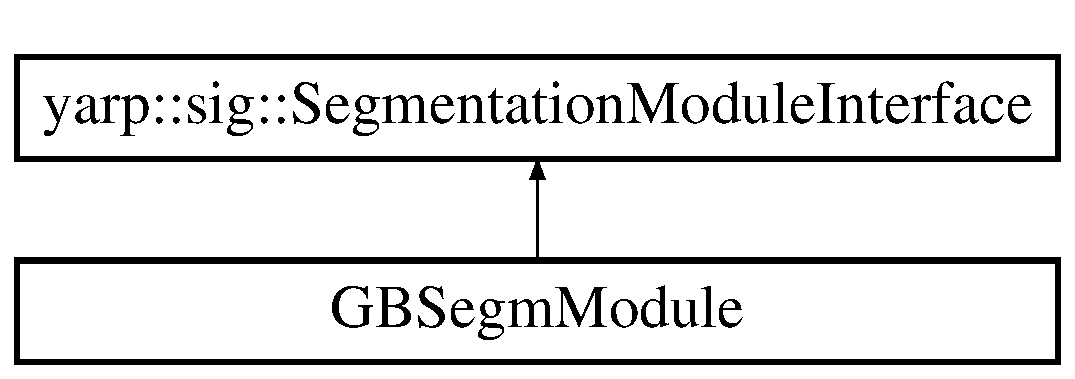
\includegraphics[height=2.000000cm]{classGBSegmModule}
\end{center}
\end{figure}
\subsection*{Public Member Functions}
\begin{DoxyCompactItemize}
\item 
\mbox{\label{classGBSegmModule_ada22cbfc66dd9b75a7a824e1ce642639}} 
virtual bool {\bfseries configure} (yarp\+::os\+::\+Resource\+Finder \&rf)
\item 
\mbox{\label{classGBSegmModule_ac3259b29883674bf47aa962f54806913}} 
virtual bool {\bfseries close} ()
\item 
\mbox{\label{classGBSegmModule_a99b9908ade3135dd5ee491b799d5e171}} 
virtual bool {\bfseries interrupt\+Module} ()
\item 
\mbox{\label{classGBSegmModule_a66f40b6ae480a039a2c10f6b91c59dde}} 
virtual bool {\bfseries update\+Module} ()
\item 
\mbox{\label{classGBSegmModule_a4ae8d5fee391d799299a10e09a5ea8c4}} 
bool {\bfseries attach} (yarp\+::os\+::\+Port \&source)
\item 
virtual void \hyperlink{classGBSegmModule_a27ffe08d394d321d9f9441423d36ef5e}{set\+\_\+sigma} (const double new\+Value)
\begin{DoxyCompactList}\small\item\em Set sigma (smoothing) parameter for the algorithm. \end{DoxyCompactList}\item 
virtual void \hyperlink{classGBSegmModule_a15129913273e221a46c428f697e40575}{set\+\_\+k} (const double new\+Value)
\begin{DoxyCompactList}\small\item\em Set k (scale factor for boundary-\/detection threshold function) parameter for the algorithm. \end{DoxyCompactList}\item 
virtual void \hyperlink{classGBSegmModule_ae1c722c9c774cbde4f6bfada3f0826ba}{set\+\_\+min\+Region} (const double new\+Value)
\begin{DoxyCompactList}\small\item\em Set min\+Region parameter for the algorithm, i.\+e., the minimum size of any segmented component. \end{DoxyCompactList}\item 
virtual double \hyperlink{classGBSegmModule_ae32ae1b1461e19c3a1b2f429c729ed03}{get\+\_\+sigma} ()
\begin{DoxyCompactList}\small\item\em Get sigma (smoothing) parameter for the algorithm. \end{DoxyCompactList}\item 
virtual double \hyperlink{classGBSegmModule_a44bab99aa7a035e57a185673c040d2f6}{get\+\_\+k} ()
\begin{DoxyCompactList}\small\item\em Get k (scale factor for boundary-\/detection threshold function) parameter for the algorithm. \end{DoxyCompactList}\item 
virtual double \hyperlink{classGBSegmModule_a2378b95e60b406a119947aa86b5bb9c4}{get\+\_\+min\+Region} ()
\begin{DoxyCompactList}\small\item\em Get min\+Region parameter for the algorithm, i.\+e., the minimum size of any segmented component. \end{DoxyCompactList}\item 
virtual int32\+\_\+t \hyperlink{classGBSegmModule_a655ee7c895eed07b07099133b9d8ce68}{get\+\_\+num\+\_\+components} ()
\begin{DoxyCompactList}\small\item\em Get the number of segmented components that have been detected in the last provided image. \end{DoxyCompactList}\item 
virtual std\+::vector$<$ \hyperlink{classyarp_1_1sig_1_1Pixel}{yarp\+::sig\+::\+Pixel} $>$ \hyperlink{classGBSegmModule_a0b63c53513e67c4f126e29cf7f28ad53}{get\+\_\+component\+\_\+around} (const \hyperlink{classyarp_1_1sig_1_1Pixel}{yarp\+::sig\+::\+Pixel} \&obj\+Center)
\begin{DoxyCompactList}\small\item\em Get the list of pixels corresponding to the component to which a given pixel belongs. \end{DoxyCompactList}\item 
\mbox{\label{classyarp_1_1sig_1_1SegmentationModuleInterface_a8ed15458e768ad8dcc58b622a6f1d282}} 
virtual bool {\bfseries read} (yarp\+::os\+::\+Connection\+Reader \&connection) Y\+A\+R\+P\+\_\+\+O\+V\+E\+R\+R\+I\+DE
\item 
\mbox{\label{classyarp_1_1sig_1_1SegmentationModuleInterface_a14ea1dff9efc91a5099633740b3e45f9}} 
virtual std\+::vector$<$ std\+::string $>$ {\bfseries help} (const std\+::string \&function\+Name=\char`\"{}-\/-\/all\char`\"{})
\end{DoxyCompactItemize}


\subsection{Detailed Description}
Segmentation Module. 



Definition at line 30 of file Segm\+Module.\+h.



\subsection{Member Function Documentation}
\mbox{\label{classGBSegmModule_a0b63c53513e67c4f126e29cf7f28ad53}} 
\index{G\+B\+Segm\+Module@{G\+B\+Segm\+Module}!get\+\_\+component\+\_\+around@{get\+\_\+component\+\_\+around}}
\index{get\+\_\+component\+\_\+around@{get\+\_\+component\+\_\+around}!G\+B\+Segm\+Module@{G\+B\+Segm\+Module}}
\subsubsection{\texorpdfstring{get\+\_\+component\+\_\+around()}{get\_component\_around()}}
{\footnotesize\ttfamily std\+::vector$<$ \hyperlink{classyarp_1_1sig_1_1Pixel}{Pixel} $>$ G\+B\+Segm\+Module\+::get\+\_\+component\+\_\+around (\begin{DoxyParamCaption}\item[{const \hyperlink{classyarp_1_1sig_1_1Pixel}{yarp\+::sig\+::\+Pixel} \&}]{obj\+Center }\end{DoxyParamCaption})\hspace{0.3cm}{\ttfamily [virtual]}}



Get the list of pixels corresponding to the component to which a given pixel belongs. 


\begin{DoxyParams}{Parameters}
{\em obj\+Center} & a pixel belonging to the region of interest \\
\hline
\end{DoxyParams}
\begin{DoxyReturn}{Returns}
list of pixels belonging to the same component as the input pixels 
\end{DoxyReturn}


Reimplemented from \hyperlink{classyarp_1_1sig_1_1SegmentationModuleInterface_a9bf0b95fbab216b2284122b0b8a36820}{yarp\+::sig\+::\+Segmentation\+Module\+Interface}.



Definition at line 71 of file Segm\+Module.\+cpp.



References yarp\+::sig\+::\+Pixel\+::x, and yarp\+::sig\+::\+Pixel\+::y.


\begin{DoxyCode}
72 \{
73     vector<Pixel> result;
74     result.clear();
75     segMutex.wait();
76     rgb componentColor = imRef(seg, objCenter.x, objCenter.y);
77     \textcolor{keywordflow}{for} (\textcolor{keywordtype}{int} y = 0; y < seg->height(); y++) \{
78 
79             \textcolor{keywordflow}{for} (\textcolor{keywordtype}{int} x = 0; x < seg->width(); x++) \{
80 
81               \textcolor{keywordflow}{if} (imRef(seg, x, y) == componentColor)
82                 result.push\_back(Pixel(x, y));
83 
84 
85             \}
86 
87         \}
88 
89     
90     segMutex.post();
91     \textcolor{keywordflow}{return} result;
92 
93 \}
\end{DoxyCode}
\mbox{\label{classGBSegmModule_a44bab99aa7a035e57a185673c040d2f6}} 
\index{G\+B\+Segm\+Module@{G\+B\+Segm\+Module}!get\+\_\+k@{get\+\_\+k}}
\index{get\+\_\+k@{get\+\_\+k}!G\+B\+Segm\+Module@{G\+B\+Segm\+Module}}
\subsubsection{\texorpdfstring{get\+\_\+k()}{get\_k()}}
{\footnotesize\ttfamily double G\+B\+Segm\+Module\+::get\+\_\+k (\begin{DoxyParamCaption}{ }\end{DoxyParamCaption})\hspace{0.3cm}{\ttfamily [virtual]}}



Get k (scale factor for boundary-\/detection threshold function) parameter for the algorithm. 

\begin{DoxyReturn}{Returns}
current value for k parameter 
\end{DoxyReturn}


Reimplemented from \hyperlink{classyarp_1_1sig_1_1SegmentationModuleInterface_a91f3d872a48599337d1d2f365ac4c31e}{yarp\+::sig\+::\+Segmentation\+Module\+Interface}.



Definition at line 68 of file Segm\+Module.\+cpp.


\begin{DoxyCode}
68 \{\textcolor{keywordflow}{return} k;\}
\end{DoxyCode}
\mbox{\label{classGBSegmModule_a2378b95e60b406a119947aa86b5bb9c4}} 
\index{G\+B\+Segm\+Module@{G\+B\+Segm\+Module}!get\+\_\+min\+Region@{get\+\_\+min\+Region}}
\index{get\+\_\+min\+Region@{get\+\_\+min\+Region}!G\+B\+Segm\+Module@{G\+B\+Segm\+Module}}
\subsubsection{\texorpdfstring{get\+\_\+min\+Region()}{get\_minRegion()}}
{\footnotesize\ttfamily double G\+B\+Segm\+Module\+::get\+\_\+min\+Region (\begin{DoxyParamCaption}{ }\end{DoxyParamCaption})\hspace{0.3cm}{\ttfamily [virtual]}}



Get min\+Region parameter for the algorithm, i.\+e., the minimum size of any segmented component. 

\begin{DoxyReturn}{Returns}
current value for min\+Region parameter 
\end{DoxyReturn}


Reimplemented from \hyperlink{classyarp_1_1sig_1_1SegmentationModuleInterface_a6c184aeea894f6afcc342c5aa748429d}{yarp\+::sig\+::\+Segmentation\+Module\+Interface}.



Definition at line 69 of file Segm\+Module.\+cpp.


\begin{DoxyCode}
69 \{\textcolor{keywordflow}{return} min\_size;\}
\end{DoxyCode}
\mbox{\label{classGBSegmModule_a655ee7c895eed07b07099133b9d8ce68}} 
\index{G\+B\+Segm\+Module@{G\+B\+Segm\+Module}!get\+\_\+num\+\_\+components@{get\+\_\+num\+\_\+components}}
\index{get\+\_\+num\+\_\+components@{get\+\_\+num\+\_\+components}!G\+B\+Segm\+Module@{G\+B\+Segm\+Module}}
\subsubsection{\texorpdfstring{get\+\_\+num\+\_\+components()}{get\_num\_components()}}
{\footnotesize\ttfamily int32\+\_\+t G\+B\+Segm\+Module\+::get\+\_\+num\+\_\+components (\begin{DoxyParamCaption}{ }\end{DoxyParamCaption})\hspace{0.3cm}{\ttfamily [virtual]}}



Get the number of segmented components that have been detected in the last provided image. 

\begin{DoxyReturn}{Returns}
number of segmented components 
\end{DoxyReturn}


Reimplemented from \hyperlink{classyarp_1_1sig_1_1SegmentationModuleInterface_a3c6b695fbef9e6827e7dd6b4cbbc38fe}{yarp\+::sig\+::\+Segmentation\+Module\+Interface}.



Definition at line 70 of file Segm\+Module.\+cpp.


\begin{DoxyCode}
70 \{\textcolor{keywordflow}{return} num\_components;\}
\end{DoxyCode}
\mbox{\label{classGBSegmModule_ae32ae1b1461e19c3a1b2f429c729ed03}} 
\index{G\+B\+Segm\+Module@{G\+B\+Segm\+Module}!get\+\_\+sigma@{get\+\_\+sigma}}
\index{get\+\_\+sigma@{get\+\_\+sigma}!G\+B\+Segm\+Module@{G\+B\+Segm\+Module}}
\subsubsection{\texorpdfstring{get\+\_\+sigma()}{get\_sigma()}}
{\footnotesize\ttfamily double G\+B\+Segm\+Module\+::get\+\_\+sigma (\begin{DoxyParamCaption}{ }\end{DoxyParamCaption})\hspace{0.3cm}{\ttfamily [virtual]}}



Get sigma (smoothing) parameter for the algorithm. 

\begin{DoxyReturn}{Returns}
current value for sigma parameter 
\end{DoxyReturn}


Reimplemented from \hyperlink{classyarp_1_1sig_1_1SegmentationModuleInterface_a38431f2c63d7da8ebf20adf0ed1da4fe}{yarp\+::sig\+::\+Segmentation\+Module\+Interface}.



Definition at line 67 of file Segm\+Module.\+cpp.


\begin{DoxyCode}
67 \{\textcolor{keywordflow}{return} sigma;\}
\end{DoxyCode}
\mbox{\label{classGBSegmModule_a15129913273e221a46c428f697e40575}} 
\index{G\+B\+Segm\+Module@{G\+B\+Segm\+Module}!set\+\_\+k@{set\+\_\+k}}
\index{set\+\_\+k@{set\+\_\+k}!G\+B\+Segm\+Module@{G\+B\+Segm\+Module}}
\subsubsection{\texorpdfstring{set\+\_\+k()}{set\_k()}}
{\footnotesize\ttfamily void G\+B\+Segm\+Module\+::set\+\_\+k (\begin{DoxyParamCaption}\item[{const double}]{new\+Value }\end{DoxyParamCaption})\hspace{0.3cm}{\ttfamily [virtual]}}



Set k (scale factor for boundary-\/detection threshold function) parameter for the algorithm. 


\begin{DoxyParams}{Parameters}
{\em new\+Value} & new value for k parameter \\
\hline
\end{DoxyParams}


Reimplemented from \hyperlink{classyarp_1_1sig_1_1SegmentationModuleInterface_a2851eae0226ad68f41cd8b61d8bb1456}{yarp\+::sig\+::\+Segmentation\+Module\+Interface}.



Definition at line 65 of file Segm\+Module.\+cpp.


\begin{DoxyCode}
65 \{k=(float)newValue;\}
\end{DoxyCode}
\mbox{\label{classGBSegmModule_ae1c722c9c774cbde4f6bfada3f0826ba}} 
\index{G\+B\+Segm\+Module@{G\+B\+Segm\+Module}!set\+\_\+min\+Region@{set\+\_\+min\+Region}}
\index{set\+\_\+min\+Region@{set\+\_\+min\+Region}!G\+B\+Segm\+Module@{G\+B\+Segm\+Module}}
\subsubsection{\texorpdfstring{set\+\_\+min\+Region()}{set\_minRegion()}}
{\footnotesize\ttfamily void G\+B\+Segm\+Module\+::set\+\_\+min\+Region (\begin{DoxyParamCaption}\item[{const double}]{new\+Value }\end{DoxyParamCaption})\hspace{0.3cm}{\ttfamily [virtual]}}



Set min\+Region parameter for the algorithm, i.\+e., the minimum size of any segmented component. 


\begin{DoxyParams}{Parameters}
{\em new\+Value} & new value for min\+Region parameter \\
\hline
\end{DoxyParams}


Reimplemented from \hyperlink{classyarp_1_1sig_1_1SegmentationModuleInterface_ad9d90ed7e362ae83e2145445a9c4301e}{yarp\+::sig\+::\+Segmentation\+Module\+Interface}.



Definition at line 66 of file Segm\+Module.\+cpp.


\begin{DoxyCode}
66 \{min\_size=(int)newValue;\}
\end{DoxyCode}
\mbox{\label{classGBSegmModule_a27ffe08d394d321d9f9441423d36ef5e}} 
\index{G\+B\+Segm\+Module@{G\+B\+Segm\+Module}!set\+\_\+sigma@{set\+\_\+sigma}}
\index{set\+\_\+sigma@{set\+\_\+sigma}!G\+B\+Segm\+Module@{G\+B\+Segm\+Module}}
\subsubsection{\texorpdfstring{set\+\_\+sigma()}{set\_sigma()}}
{\footnotesize\ttfamily void G\+B\+Segm\+Module\+::set\+\_\+sigma (\begin{DoxyParamCaption}\item[{const double}]{new\+Value }\end{DoxyParamCaption})\hspace{0.3cm}{\ttfamily [virtual]}}



Set sigma (smoothing) parameter for the algorithm. 


\begin{DoxyParams}{Parameters}
{\em new\+Value} & new value for sigma parameter \\
\hline
\end{DoxyParams}


Reimplemented from \hyperlink{classyarp_1_1sig_1_1SegmentationModuleInterface_a68f28930df5e930934c0ee56ad1f680c}{yarp\+::sig\+::\+Segmentation\+Module\+Interface}.



Definition at line 64 of file Segm\+Module.\+cpp.


\begin{DoxyCode}
64 \{sigma=(float)newValue;\}
\end{DoxyCode}


The documentation for this class was generated from the following files\+:\begin{DoxyCompactItemize}
\item 
C\+:/dev/icub-\/contrib-\/iit/segmentation/graph\+Based/Segm\+Module.\+h\item 
C\+:/dev/icub-\/contrib-\/iit/segmentation/graph\+Based/Segm\+Module.\+cpp\end{DoxyCompactItemize}

\section{lbp\+Extract\+\_\+\+I\+D\+L\+Server Class Reference}
\label{classlbpExtract__IDLServer}\index{lbp\+Extract\+\_\+\+I\+D\+L\+Server@{lbp\+Extract\+\_\+\+I\+D\+L\+Server}}


\hyperlink{classlbpExtract__IDLServer}{lbp\+Extract\+\_\+\+I\+D\+L\+Server} Interface.  




{\ttfamily \#include $<$lbp\+Extract\+\_\+\+I\+D\+L\+Server.\+h$>$}



Inherits Wire.



Inherited by S\+E\+G\+M\+E\+N\+T\+Module.

\subsection*{Public Member Functions}
\begin{DoxyCompactItemize}
\item 
virtual bool \hyperlink{classlbpExtract__IDLServer_a9d9b1223c68851e94b0c8c0bd8d3cedc}{reset} ()
\begin{DoxyCompactList}\small\item\em Resets all the histograms. \end{DoxyCompactList}\item 
virtual bool \hyperlink{classlbpExtract__IDLServer_a4086feb2a3cee548670673235277b6f0}{quit} ()
\begin{DoxyCompactList}\small\item\em Quit the module. \end{DoxyCompactList}\item 
virtual bool \hyperlink{classlbpExtract__IDLServer_a2391f554973a3b7d32d6eea6bbb233d7}{set\+Radius} (const int32\+\_\+t radius)
\begin{DoxyCompactList}\small\item\em Sets the radius of the lbp operators. \end{DoxyCompactList}\item 
virtual int32\+\_\+t \hyperlink{classlbpExtract__IDLServer_a8c9a3adfcb9e7d37c4388bc3950da23b}{get\+Radius} ()
\begin{DoxyCompactList}\small\item\em Gets the radius of the lbp operators. \end{DoxyCompactList}\item 
virtual bool \hyperlink{classlbpExtract__IDLServer_aa72b58e41cf97d26825515cc9d5e6aa6}{set\+Neighbours} (const int32\+\_\+t neighbours)
\begin{DoxyCompactList}\small\item\em Sets the neighbours value of the lbp operators. \end{DoxyCompactList}\item 
virtual int32\+\_\+t \hyperlink{classlbpExtract__IDLServer_abf7693b9f3f63c2a16e163a3991b7d01}{get\+Neighbours} ()
\begin{DoxyCompactList}\small\item\em Gets the neighbours of the lbp operators. \end{DoxyCompactList}\item 
virtual int32\+\_\+t \hyperlink{classlbpExtract__IDLServer_a693ea8bf9638a27fdf3f7d40f7ad8f51}{get\+Top\+Bound} ()
\begin{DoxyCompactList}\small\item\em Gets the top bound (Y) limit for the blobs. \end{DoxyCompactList}\item 
virtual bool \hyperlink{classlbpExtract__IDLServer_a50677882bf32262601b91046a2dcdbf2}{set\+Top\+Bound} (const int32\+\_\+t top\+Bound)
\begin{DoxyCompactList}\small\item\em Sets the top bound (Y) limit for the blobs. \end{DoxyCompactList}\item 
virtual int32\+\_\+t \hyperlink{classlbpExtract__IDLServer_ae98976e14296fd7fd3596da8faf862d3}{get\+Min\+Arc\+Length} ()
\begin{DoxyCompactList}\small\item\em Gets the minimum arc length of the allowed blobs. \end{DoxyCompactList}\item 
virtual bool \hyperlink{classlbpExtract__IDLServer_abd1ebed4459c05a4b849f8eebea14127}{set\+Min\+Arc\+Length} (const int32\+\_\+t min\+Arc\+Length)
\begin{DoxyCompactList}\small\item\em Sets the minimum arc length of the allowed blobs. \end{DoxyCompactList}\item 
virtual int32\+\_\+t \hyperlink{classlbpExtract__IDLServer_ae6f220a2b984c7211bd59beca4db0373}{get\+Max\+Arc\+Length} ()
\begin{DoxyCompactList}\small\item\em Gets the maximum arc length of the allowed blobs. \end{DoxyCompactList}\item 
virtual bool \hyperlink{classlbpExtract__IDLServer_abc379ba01952949df03f977c74884ade}{set\+Max\+Arc\+Length} (const int32\+\_\+t max\+Arc\+Length)
\begin{DoxyCompactList}\small\item\em Sets the maximum arc length of the allowed blobs. \end{DoxyCompactList}\item 
virtual int32\+\_\+t \hyperlink{classlbpExtract__IDLServer_a46c4f38052cd2abd334e4e0f0263fab4}{get\+Max\+Area} ()
\begin{DoxyCompactList}\small\item\em Gets the maximum area of the allowed blobs. \end{DoxyCompactList}\item 
virtual bool \hyperlink{classlbpExtract__IDLServer_a81dbd91a1460cdb450a7f7824e6d9953}{set\+Max\+Area} (const int32\+\_\+t max\+Area)
\begin{DoxyCompactList}\small\item\em Sets the maximum area of the allowed blobs. \end{DoxyCompactList}\item 
virtual int32\+\_\+t \hyperlink{classlbpExtract__IDLServer_a3f6f2aba33eeb0a15d73fdfc5817ef7a}{get\+Min\+Area} ()
\begin{DoxyCompactList}\small\item\em Gets the minimum area of the allowed blobs. \end{DoxyCompactList}\item 
virtual bool \hyperlink{classlbpExtract__IDLServer_a13eb918e54b2eee6fe2811fbe8f6aee6}{set\+Min\+Area} (const int32\+\_\+t min\+Area)
\begin{DoxyCompactList}\small\item\em Sets the minimum area of the allowed blobs. \end{DoxyCompactList}\item 
virtual int32\+\_\+t \hyperlink{classlbpExtract__IDLServer_a48094f72a89aa3218e3449dfe071f0f7}{get\+Num\+Iteration} ()
\begin{DoxyCompactList}\small\item\em Gets the number of iteration for the grab\+Cut segmentation algorithm. \end{DoxyCompactList}\item 
virtual bool \hyperlink{classlbpExtract__IDLServer_a2955fa69c12b59a03c2b1e130747b054}{set\+Num\+Iteration} (const int32\+\_\+t num\+Iteration)
\begin{DoxyCompactList}\small\item\em Sets the number of iteration for the grab\+Cut segmentation algorithm. \end{DoxyCompactList}\item 
virtual bool \hyperlink{classlbpExtract__IDLServer_a88f2492af4a66eaf9be8ceb28c862fe5}{reset\+All\+Values} ()
\begin{DoxyCompactList}\small\item\em resets all values to the default ones. \end{DoxyCompactList}\item 
virtual bool \hyperlink{classlbpExtract__IDLServer_aebf9bfaa7a16309244177c4b7b094e2a}{setbb\+Offset} (const int32\+\_\+t offset)
\begin{DoxyCompactList}\small\item\em Sets the offset of the bounding box. \end{DoxyCompactList}\item 
virtual int32\+\_\+t \hyperlink{classlbpExtract__IDLServer_a2260626a2137fc9ffe9364fad3444024}{getbb\+Offset} ()
\begin{DoxyCompactList}\small\item\em Gets the current offset of the bounding box. \end{DoxyCompactList}\item 
virtual bool \hyperlink{classlbpExtract__IDLServer_a1b9021d363199f1a334c7ec2c23801b1}{verbosity} (const int32\+\_\+t bool\+Verbosity)
\begin{DoxyCompactList}\small\item\em Sets the verbosity of the algorithm. \end{DoxyCompactList}\item 
virtual yarp\+::os\+::\+Bottle \hyperlink{classlbpExtract__IDLServer_a9d92e9eba6c2ea72a43b1c8077bc6d0a}{get\+\_\+component\+\_\+around} (const int32\+\_\+t x, const int32\+\_\+t y)
\begin{DoxyCompactList}\small\item\em Gets all the components (points) that belong to any of the segmented blobs. \end{DoxyCompactList}\item 
\mbox{\label{classlbpExtract__IDLServer_a677697653e78ed82aaa6543eb875bd41}} 
virtual bool {\bfseries read} (yarp\+::os\+::\+Connection\+Reader \&connection)
\item 
\mbox{\label{classlbpExtract__IDLServer_a13b6fbd034b38f4b5879381dabad05ed}} 
virtual std\+::vector$<$ std\+::string $>$ {\bfseries help} (const std\+::string \&function\+Name=\char`\"{}-\/-\/all\char`\"{})
\end{DoxyCompactItemize}


\subsection{Detailed Description}
\hyperlink{classlbpExtract__IDLServer}{lbp\+Extract\+\_\+\+I\+D\+L\+Server} Interface. 

Definition at line 18 of file lbp\+Extract\+\_\+\+I\+D\+L\+Server.\+h.



\subsection{Member Function Documentation}
\mbox{\label{classlbpExtract__IDLServer_a9d92e9eba6c2ea72a43b1c8077bc6d0a}} 
\index{lbp\+Extract\+\_\+\+I\+D\+L\+Server@{lbp\+Extract\+\_\+\+I\+D\+L\+Server}!get\+\_\+component\+\_\+around@{get\+\_\+component\+\_\+around}}
\index{get\+\_\+component\+\_\+around@{get\+\_\+component\+\_\+around}!lbp\+Extract\+\_\+\+I\+D\+L\+Server@{lbp\+Extract\+\_\+\+I\+D\+L\+Server}}
\subsubsection{\texorpdfstring{get\+\_\+component\+\_\+around()}{get\_component\_around()}}
{\footnotesize\ttfamily virtual yarp\+::os\+::\+Bottle lbp\+Extract\+\_\+\+I\+D\+L\+Server\+::get\+\_\+component\+\_\+around (\begin{DoxyParamCaption}\item[{const int32\+\_\+t}]{x,  }\item[{const int32\+\_\+t}]{y }\end{DoxyParamCaption})\hspace{0.3cm}{\ttfamily [virtual]}}



Gets all the components (points) that belong to any of the segmented blobs. 


\begin{DoxyParams}{Parameters}
{\em x} & x coordinate of seed point \\
\hline
{\em y} & y coordinate of seed point \\
\hline
\end{DoxyParams}
\begin{DoxyReturn}{Returns}
Bottle containing a list of points belonging to the segmented blob 
\end{DoxyReturn}
\mbox{\label{classlbpExtract__IDLServer_a2260626a2137fc9ffe9364fad3444024}} 
\index{lbp\+Extract\+\_\+\+I\+D\+L\+Server@{lbp\+Extract\+\_\+\+I\+D\+L\+Server}!getbb\+Offset@{getbb\+Offset}}
\index{getbb\+Offset@{getbb\+Offset}!lbp\+Extract\+\_\+\+I\+D\+L\+Server@{lbp\+Extract\+\_\+\+I\+D\+L\+Server}}
\subsubsection{\texorpdfstring{getbb\+Offset()}{getbbOffset()}}
{\footnotesize\ttfamily virtual int32\+\_\+t lbp\+Extract\+\_\+\+I\+D\+L\+Server\+::getbb\+Offset (\begin{DoxyParamCaption}{ }\end{DoxyParamCaption})\hspace{0.3cm}{\ttfamily [virtual]}}



Gets the current offset of the bounding box. 

\begin{DoxyReturn}{Returns}
true/false on success/failure 
\end{DoxyReturn}
\mbox{\label{classlbpExtract__IDLServer_ae6f220a2b984c7211bd59beca4db0373}} 
\index{lbp\+Extract\+\_\+\+I\+D\+L\+Server@{lbp\+Extract\+\_\+\+I\+D\+L\+Server}!get\+Max\+Arc\+Length@{get\+Max\+Arc\+Length}}
\index{get\+Max\+Arc\+Length@{get\+Max\+Arc\+Length}!lbp\+Extract\+\_\+\+I\+D\+L\+Server@{lbp\+Extract\+\_\+\+I\+D\+L\+Server}}
\subsubsection{\texorpdfstring{get\+Max\+Arc\+Length()}{getMaxArcLength()}}
{\footnotesize\ttfamily virtual int32\+\_\+t lbp\+Extract\+\_\+\+I\+D\+L\+Server\+::get\+Max\+Arc\+Length (\begin{DoxyParamCaption}{ }\end{DoxyParamCaption})\hspace{0.3cm}{\ttfamily [virtual]}}



Gets the maximum arc length of the allowed blobs. 

\begin{DoxyReturn}{Returns}
the current maximum arc length 
\end{DoxyReturn}
\mbox{\label{classlbpExtract__IDLServer_a46c4f38052cd2abd334e4e0f0263fab4}} 
\index{lbp\+Extract\+\_\+\+I\+D\+L\+Server@{lbp\+Extract\+\_\+\+I\+D\+L\+Server}!get\+Max\+Area@{get\+Max\+Area}}
\index{get\+Max\+Area@{get\+Max\+Area}!lbp\+Extract\+\_\+\+I\+D\+L\+Server@{lbp\+Extract\+\_\+\+I\+D\+L\+Server}}
\subsubsection{\texorpdfstring{get\+Max\+Area()}{getMaxArea()}}
{\footnotesize\ttfamily virtual int32\+\_\+t lbp\+Extract\+\_\+\+I\+D\+L\+Server\+::get\+Max\+Area (\begin{DoxyParamCaption}{ }\end{DoxyParamCaption})\hspace{0.3cm}{\ttfamily [virtual]}}



Gets the maximum area of the allowed blobs. 

\begin{DoxyReturn}{Returns}
the current maximum area 
\end{DoxyReturn}
\mbox{\label{classlbpExtract__IDLServer_ae98976e14296fd7fd3596da8faf862d3}} 
\index{lbp\+Extract\+\_\+\+I\+D\+L\+Server@{lbp\+Extract\+\_\+\+I\+D\+L\+Server}!get\+Min\+Arc\+Length@{get\+Min\+Arc\+Length}}
\index{get\+Min\+Arc\+Length@{get\+Min\+Arc\+Length}!lbp\+Extract\+\_\+\+I\+D\+L\+Server@{lbp\+Extract\+\_\+\+I\+D\+L\+Server}}
\subsubsection{\texorpdfstring{get\+Min\+Arc\+Length()}{getMinArcLength()}}
{\footnotesize\ttfamily virtual int32\+\_\+t lbp\+Extract\+\_\+\+I\+D\+L\+Server\+::get\+Min\+Arc\+Length (\begin{DoxyParamCaption}{ }\end{DoxyParamCaption})\hspace{0.3cm}{\ttfamily [virtual]}}



Gets the minimum arc length of the allowed blobs. 

\begin{DoxyReturn}{Returns}
the current minimum arc length 
\end{DoxyReturn}
\mbox{\label{classlbpExtract__IDLServer_a3f6f2aba33eeb0a15d73fdfc5817ef7a}} 
\index{lbp\+Extract\+\_\+\+I\+D\+L\+Server@{lbp\+Extract\+\_\+\+I\+D\+L\+Server}!get\+Min\+Area@{get\+Min\+Area}}
\index{get\+Min\+Area@{get\+Min\+Area}!lbp\+Extract\+\_\+\+I\+D\+L\+Server@{lbp\+Extract\+\_\+\+I\+D\+L\+Server}}
\subsubsection{\texorpdfstring{get\+Min\+Area()}{getMinArea()}}
{\footnotesize\ttfamily virtual int32\+\_\+t lbp\+Extract\+\_\+\+I\+D\+L\+Server\+::get\+Min\+Area (\begin{DoxyParamCaption}{ }\end{DoxyParamCaption})\hspace{0.3cm}{\ttfamily [virtual]}}



Gets the minimum area of the allowed blobs. 

\begin{DoxyReturn}{Returns}
the current minimum area 
\end{DoxyReturn}
\mbox{\label{classlbpExtract__IDLServer_abf7693b9f3f63c2a16e163a3991b7d01}} 
\index{lbp\+Extract\+\_\+\+I\+D\+L\+Server@{lbp\+Extract\+\_\+\+I\+D\+L\+Server}!get\+Neighbours@{get\+Neighbours}}
\index{get\+Neighbours@{get\+Neighbours}!lbp\+Extract\+\_\+\+I\+D\+L\+Server@{lbp\+Extract\+\_\+\+I\+D\+L\+Server}}
\subsubsection{\texorpdfstring{get\+Neighbours()}{getNeighbours()}}
{\footnotesize\ttfamily virtual int32\+\_\+t lbp\+Extract\+\_\+\+I\+D\+L\+Server\+::get\+Neighbours (\begin{DoxyParamCaption}{ }\end{DoxyParamCaption})\hspace{0.3cm}{\ttfamily [virtual]}}



Gets the neighbours of the lbp operators. 

\begin{DoxyReturn}{Returns}
the current radius of the lpb operator 
\end{DoxyReturn}
\mbox{\label{classlbpExtract__IDLServer_a48094f72a89aa3218e3449dfe071f0f7}} 
\index{lbp\+Extract\+\_\+\+I\+D\+L\+Server@{lbp\+Extract\+\_\+\+I\+D\+L\+Server}!get\+Num\+Iteration@{get\+Num\+Iteration}}
\index{get\+Num\+Iteration@{get\+Num\+Iteration}!lbp\+Extract\+\_\+\+I\+D\+L\+Server@{lbp\+Extract\+\_\+\+I\+D\+L\+Server}}
\subsubsection{\texorpdfstring{get\+Num\+Iteration()}{getNumIteration()}}
{\footnotesize\ttfamily virtual int32\+\_\+t lbp\+Extract\+\_\+\+I\+D\+L\+Server\+::get\+Num\+Iteration (\begin{DoxyParamCaption}{ }\end{DoxyParamCaption})\hspace{0.3cm}{\ttfamily [virtual]}}



Gets the number of iteration for the grab\+Cut segmentation algorithm. 

\begin{DoxyReturn}{Returns}
the current maximum arc length 
\end{DoxyReturn}
\mbox{\label{classlbpExtract__IDLServer_a8c9a3adfcb9e7d37c4388bc3950da23b}} 
\index{lbp\+Extract\+\_\+\+I\+D\+L\+Server@{lbp\+Extract\+\_\+\+I\+D\+L\+Server}!get\+Radius@{get\+Radius}}
\index{get\+Radius@{get\+Radius}!lbp\+Extract\+\_\+\+I\+D\+L\+Server@{lbp\+Extract\+\_\+\+I\+D\+L\+Server}}
\subsubsection{\texorpdfstring{get\+Radius()}{getRadius()}}
{\footnotesize\ttfamily virtual int32\+\_\+t lbp\+Extract\+\_\+\+I\+D\+L\+Server\+::get\+Radius (\begin{DoxyParamCaption}{ }\end{DoxyParamCaption})\hspace{0.3cm}{\ttfamily [virtual]}}



Gets the radius of the lbp operators. 

\begin{DoxyReturn}{Returns}
the current radius of the lpb operator 
\end{DoxyReturn}
\mbox{\label{classlbpExtract__IDLServer_a693ea8bf9638a27fdf3f7d40f7ad8f51}} 
\index{lbp\+Extract\+\_\+\+I\+D\+L\+Server@{lbp\+Extract\+\_\+\+I\+D\+L\+Server}!get\+Top\+Bound@{get\+Top\+Bound}}
\index{get\+Top\+Bound@{get\+Top\+Bound}!lbp\+Extract\+\_\+\+I\+D\+L\+Server@{lbp\+Extract\+\_\+\+I\+D\+L\+Server}}
\subsubsection{\texorpdfstring{get\+Top\+Bound()}{getTopBound()}}
{\footnotesize\ttfamily virtual int32\+\_\+t lbp\+Extract\+\_\+\+I\+D\+L\+Server\+::get\+Top\+Bound (\begin{DoxyParamCaption}{ }\end{DoxyParamCaption})\hspace{0.3cm}{\ttfamily [virtual]}}



Gets the top bound (Y) limit for the blobs. 

\begin{DoxyReturn}{Returns}
the current top bound limit 
\end{DoxyReturn}
\mbox{\label{classlbpExtract__IDLServer_a4086feb2a3cee548670673235277b6f0}} 
\index{lbp\+Extract\+\_\+\+I\+D\+L\+Server@{lbp\+Extract\+\_\+\+I\+D\+L\+Server}!quit@{quit}}
\index{quit@{quit}!lbp\+Extract\+\_\+\+I\+D\+L\+Server@{lbp\+Extract\+\_\+\+I\+D\+L\+Server}}
\subsubsection{\texorpdfstring{quit()}{quit()}}
{\footnotesize\ttfamily virtual bool lbp\+Extract\+\_\+\+I\+D\+L\+Server\+::quit (\begin{DoxyParamCaption}{ }\end{DoxyParamCaption})\hspace{0.3cm}{\ttfamily [virtual]}}



Quit the module. 

\begin{DoxyReturn}{Returns}
true/false on success/failure 
\end{DoxyReturn}
\mbox{\label{classlbpExtract__IDLServer_a9d9b1223c68851e94b0c8c0bd8d3cedc}} 
\index{lbp\+Extract\+\_\+\+I\+D\+L\+Server@{lbp\+Extract\+\_\+\+I\+D\+L\+Server}!reset@{reset}}
\index{reset@{reset}!lbp\+Extract\+\_\+\+I\+D\+L\+Server@{lbp\+Extract\+\_\+\+I\+D\+L\+Server}}
\subsubsection{\texorpdfstring{reset()}{reset()}}
{\footnotesize\ttfamily virtual bool lbp\+Extract\+\_\+\+I\+D\+L\+Server\+::reset (\begin{DoxyParamCaption}{ }\end{DoxyParamCaption})\hspace{0.3cm}{\ttfamily [virtual]}}



Resets all the histograms. 

\begin{DoxyReturn}{Returns}
true/false on success/failure 
\end{DoxyReturn}
\mbox{\label{classlbpExtract__IDLServer_a88f2492af4a66eaf9be8ceb28c862fe5}} 
\index{lbp\+Extract\+\_\+\+I\+D\+L\+Server@{lbp\+Extract\+\_\+\+I\+D\+L\+Server}!reset\+All\+Values@{reset\+All\+Values}}
\index{reset\+All\+Values@{reset\+All\+Values}!lbp\+Extract\+\_\+\+I\+D\+L\+Server@{lbp\+Extract\+\_\+\+I\+D\+L\+Server}}
\subsubsection{\texorpdfstring{reset\+All\+Values()}{resetAllValues()}}
{\footnotesize\ttfamily virtual bool lbp\+Extract\+\_\+\+I\+D\+L\+Server\+::reset\+All\+Values (\begin{DoxyParamCaption}{ }\end{DoxyParamCaption})\hspace{0.3cm}{\ttfamily [virtual]}}



resets all values to the default ones. 

(acts as a backup) \begin{DoxyReturn}{Returns}
true/false on success/failure 
\end{DoxyReturn}
\mbox{\label{classlbpExtract__IDLServer_aebf9bfaa7a16309244177c4b7b094e2a}} 
\index{lbp\+Extract\+\_\+\+I\+D\+L\+Server@{lbp\+Extract\+\_\+\+I\+D\+L\+Server}!setbb\+Offset@{setbb\+Offset}}
\index{setbb\+Offset@{setbb\+Offset}!lbp\+Extract\+\_\+\+I\+D\+L\+Server@{lbp\+Extract\+\_\+\+I\+D\+L\+Server}}
\subsubsection{\texorpdfstring{setbb\+Offset()}{setbbOffset()}}
{\footnotesize\ttfamily virtual bool lbp\+Extract\+\_\+\+I\+D\+L\+Server\+::setbb\+Offset (\begin{DoxyParamCaption}\item[{const int32\+\_\+t}]{offset }\end{DoxyParamCaption})\hspace{0.3cm}{\ttfamily [virtual]}}



Sets the offset of the bounding box. 

This increases the size of the bb to add more backgound \begin{DoxyReturn}{Returns}
true/false on success/failure 
\end{DoxyReturn}
\mbox{\label{classlbpExtract__IDLServer_abc379ba01952949df03f977c74884ade}} 
\index{lbp\+Extract\+\_\+\+I\+D\+L\+Server@{lbp\+Extract\+\_\+\+I\+D\+L\+Server}!set\+Max\+Arc\+Length@{set\+Max\+Arc\+Length}}
\index{set\+Max\+Arc\+Length@{set\+Max\+Arc\+Length}!lbp\+Extract\+\_\+\+I\+D\+L\+Server@{lbp\+Extract\+\_\+\+I\+D\+L\+Server}}
\subsubsection{\texorpdfstring{set\+Max\+Arc\+Length()}{setMaxArcLength()}}
{\footnotesize\ttfamily virtual bool lbp\+Extract\+\_\+\+I\+D\+L\+Server\+::set\+Max\+Arc\+Length (\begin{DoxyParamCaption}\item[{const int32\+\_\+t}]{max\+Arc\+Length }\end{DoxyParamCaption})\hspace{0.3cm}{\ttfamily [virtual]}}



Sets the maximum arc length of the allowed blobs. 


\begin{DoxyParams}{Parameters}
{\em max\+Arc\+Length,integer} & containing the max\+Arc\+Length \\
\hline
\end{DoxyParams}
\begin{DoxyReturn}{Returns}
true/false on success/failure 
\end{DoxyReturn}
\mbox{\label{classlbpExtract__IDLServer_a81dbd91a1460cdb450a7f7824e6d9953}} 
\index{lbp\+Extract\+\_\+\+I\+D\+L\+Server@{lbp\+Extract\+\_\+\+I\+D\+L\+Server}!set\+Max\+Area@{set\+Max\+Area}}
\index{set\+Max\+Area@{set\+Max\+Area}!lbp\+Extract\+\_\+\+I\+D\+L\+Server@{lbp\+Extract\+\_\+\+I\+D\+L\+Server}}
\subsubsection{\texorpdfstring{set\+Max\+Area()}{setMaxArea()}}
{\footnotesize\ttfamily virtual bool lbp\+Extract\+\_\+\+I\+D\+L\+Server\+::set\+Max\+Area (\begin{DoxyParamCaption}\item[{const int32\+\_\+t}]{max\+Area }\end{DoxyParamCaption})\hspace{0.3cm}{\ttfamily [virtual]}}



Sets the maximum area of the allowed blobs. 


\begin{DoxyParams}{Parameters}
{\em max\+Area,integer} & containing the max\+Area \\
\hline
\end{DoxyParams}
\begin{DoxyReturn}{Returns}
true/false on success/failure 
\end{DoxyReturn}
\mbox{\label{classlbpExtract__IDLServer_abd1ebed4459c05a4b849f8eebea14127}} 
\index{lbp\+Extract\+\_\+\+I\+D\+L\+Server@{lbp\+Extract\+\_\+\+I\+D\+L\+Server}!set\+Min\+Arc\+Length@{set\+Min\+Arc\+Length}}
\index{set\+Min\+Arc\+Length@{set\+Min\+Arc\+Length}!lbp\+Extract\+\_\+\+I\+D\+L\+Server@{lbp\+Extract\+\_\+\+I\+D\+L\+Server}}
\subsubsection{\texorpdfstring{set\+Min\+Arc\+Length()}{setMinArcLength()}}
{\footnotesize\ttfamily virtual bool lbp\+Extract\+\_\+\+I\+D\+L\+Server\+::set\+Min\+Arc\+Length (\begin{DoxyParamCaption}\item[{const int32\+\_\+t}]{min\+Arc\+Length }\end{DoxyParamCaption})\hspace{0.3cm}{\ttfamily [virtual]}}



Sets the minimum arc length of the allowed blobs. 


\begin{DoxyParams}{Parameters}
{\em min\+Arc\+Length,integer} & containing the min\+Arc\+Length \\
\hline
\end{DoxyParams}
\begin{DoxyReturn}{Returns}
true/false on success/failure 
\end{DoxyReturn}
\mbox{\label{classlbpExtract__IDLServer_a13eb918e54b2eee6fe2811fbe8f6aee6}} 
\index{lbp\+Extract\+\_\+\+I\+D\+L\+Server@{lbp\+Extract\+\_\+\+I\+D\+L\+Server}!set\+Min\+Area@{set\+Min\+Area}}
\index{set\+Min\+Area@{set\+Min\+Area}!lbp\+Extract\+\_\+\+I\+D\+L\+Server@{lbp\+Extract\+\_\+\+I\+D\+L\+Server}}
\subsubsection{\texorpdfstring{set\+Min\+Area()}{setMinArea()}}
{\footnotesize\ttfamily virtual bool lbp\+Extract\+\_\+\+I\+D\+L\+Server\+::set\+Min\+Area (\begin{DoxyParamCaption}\item[{const int32\+\_\+t}]{min\+Area }\end{DoxyParamCaption})\hspace{0.3cm}{\ttfamily [virtual]}}



Sets the minimum area of the allowed blobs. 


\begin{DoxyParams}{Parameters}
{\em min\+Area,integer} & containing the min\+Area \\
\hline
\end{DoxyParams}
\begin{DoxyReturn}{Returns}
true/false on success/failure 
\end{DoxyReturn}
\mbox{\label{classlbpExtract__IDLServer_aa72b58e41cf97d26825515cc9d5e6aa6}} 
\index{lbp\+Extract\+\_\+\+I\+D\+L\+Server@{lbp\+Extract\+\_\+\+I\+D\+L\+Server}!set\+Neighbours@{set\+Neighbours}}
\index{set\+Neighbours@{set\+Neighbours}!lbp\+Extract\+\_\+\+I\+D\+L\+Server@{lbp\+Extract\+\_\+\+I\+D\+L\+Server}}
\subsubsection{\texorpdfstring{set\+Neighbours()}{setNeighbours()}}
{\footnotesize\ttfamily virtual bool lbp\+Extract\+\_\+\+I\+D\+L\+Server\+::set\+Neighbours (\begin{DoxyParamCaption}\item[{const int32\+\_\+t}]{neighbours }\end{DoxyParamCaption})\hspace{0.3cm}{\ttfamily [virtual]}}



Sets the neighbours value of the lbp operators. 


\begin{DoxyParams}{Parameters}
{\em neighbours} & integer containing the number of neighbours \\
\hline
\end{DoxyParams}
\begin{DoxyReturn}{Returns}
true/false on success/failure 
\end{DoxyReturn}
\mbox{\label{classlbpExtract__IDLServer_a2955fa69c12b59a03c2b1e130747b054}} 
\index{lbp\+Extract\+\_\+\+I\+D\+L\+Server@{lbp\+Extract\+\_\+\+I\+D\+L\+Server}!set\+Num\+Iteration@{set\+Num\+Iteration}}
\index{set\+Num\+Iteration@{set\+Num\+Iteration}!lbp\+Extract\+\_\+\+I\+D\+L\+Server@{lbp\+Extract\+\_\+\+I\+D\+L\+Server}}
\subsubsection{\texorpdfstring{set\+Num\+Iteration()}{setNumIteration()}}
{\footnotesize\ttfamily virtual bool lbp\+Extract\+\_\+\+I\+D\+L\+Server\+::set\+Num\+Iteration (\begin{DoxyParamCaption}\item[{const int32\+\_\+t}]{num\+Iteration }\end{DoxyParamCaption})\hspace{0.3cm}{\ttfamily [virtual]}}



Sets the number of iteration for the grab\+Cut segmentation algorithm. 


\begin{DoxyParams}{Parameters}
{\em num\+Iteration} & \\
\hline
\end{DoxyParams}
\begin{DoxyReturn}{Returns}
true/false on success/failure 
\end{DoxyReturn}
\mbox{\label{classlbpExtract__IDLServer_a2391f554973a3b7d32d6eea6bbb233d7}} 
\index{lbp\+Extract\+\_\+\+I\+D\+L\+Server@{lbp\+Extract\+\_\+\+I\+D\+L\+Server}!set\+Radius@{set\+Radius}}
\index{set\+Radius@{set\+Radius}!lbp\+Extract\+\_\+\+I\+D\+L\+Server@{lbp\+Extract\+\_\+\+I\+D\+L\+Server}}
\subsubsection{\texorpdfstring{set\+Radius()}{setRadius()}}
{\footnotesize\ttfamily virtual bool lbp\+Extract\+\_\+\+I\+D\+L\+Server\+::set\+Radius (\begin{DoxyParamCaption}\item[{const int32\+\_\+t}]{radius }\end{DoxyParamCaption})\hspace{0.3cm}{\ttfamily [virtual]}}



Sets the radius of the lbp operators. 


\begin{DoxyParams}{Parameters}
{\em radius} & integer containing the radius \\
\hline
\end{DoxyParams}
\begin{DoxyReturn}{Returns}
true/false on success/failure 
\end{DoxyReturn}
\mbox{\label{classlbpExtract__IDLServer_a50677882bf32262601b91046a2dcdbf2}} 
\index{lbp\+Extract\+\_\+\+I\+D\+L\+Server@{lbp\+Extract\+\_\+\+I\+D\+L\+Server}!set\+Top\+Bound@{set\+Top\+Bound}}
\index{set\+Top\+Bound@{set\+Top\+Bound}!lbp\+Extract\+\_\+\+I\+D\+L\+Server@{lbp\+Extract\+\_\+\+I\+D\+L\+Server}}
\subsubsection{\texorpdfstring{set\+Top\+Bound()}{setTopBound()}}
{\footnotesize\ttfamily virtual bool lbp\+Extract\+\_\+\+I\+D\+L\+Server\+::set\+Top\+Bound (\begin{DoxyParamCaption}\item[{const int32\+\_\+t}]{top\+Bound }\end{DoxyParamCaption})\hspace{0.3cm}{\ttfamily [virtual]}}



Sets the top bound (Y) limit for the blobs. 


\begin{DoxyParams}{Parameters}
{\em top\+Bound,integer} & containing the top\+Bound \\
\hline
\end{DoxyParams}
\begin{DoxyReturn}{Returns}
true/false on success/failure 
\end{DoxyReturn}
\mbox{\label{classlbpExtract__IDLServer_a1b9021d363199f1a334c7ec2c23801b1}} 
\index{lbp\+Extract\+\_\+\+I\+D\+L\+Server@{lbp\+Extract\+\_\+\+I\+D\+L\+Server}!verbosity@{verbosity}}
\index{verbosity@{verbosity}!lbp\+Extract\+\_\+\+I\+D\+L\+Server@{lbp\+Extract\+\_\+\+I\+D\+L\+Server}}
\subsubsection{\texorpdfstring{verbosity()}{verbosity()}}
{\footnotesize\ttfamily virtual bool lbp\+Extract\+\_\+\+I\+D\+L\+Server\+::verbosity (\begin{DoxyParamCaption}\item[{const int32\+\_\+t}]{bool\+Verbosity }\end{DoxyParamCaption})\hspace{0.3cm}{\ttfamily [virtual]}}



Sets the verbosity of the algorithm. 


\begin{DoxyParams}{Parameters}
{\em bool\+Verbosity} & \\
\hline
\end{DoxyParams}
\begin{DoxyReturn}{Returns}
true/false on success/failure 
\end{DoxyReturn}


The documentation for this class was generated from the following file\+:\begin{DoxyCompactItemize}
\item 
C\+:/dev/icub-\/contrib-\/iit/segmentation/lbp\+Extract/idl\+\_\+dox/lbp\+Extract\+\_\+\+I\+D\+L\+Server.\+h\end{DoxyCompactItemize}

\section{yarp\+:\+:sig\+:\+:Pixel Class Reference}
\label{classyarp_1_1sig_1_1Pixel}\index{yarp\+::sig\+::\+Pixel@{yarp\+::sig\+::\+Pixel}}


\hyperlink{classyarp_1_1sig_1_1Pixel}{Pixel} position in the image frame.  




{\ttfamily \#include $<$Pixel.\+h$>$}



Inherits Wire\+Portable.

\subsection*{Public Types}
\begin{DoxyCompactItemize}
\item 
\mbox{\label{classyarp_1_1sig_1_1Pixel_a2e2e4781602885250c9284572e128ec5}} 
typedef yarp\+::os\+::idl\+::\+Unwrapped$<$ \hyperlink{classyarp_1_1sig_1_1Pixel}{yarp\+::sig\+::\+Pixel} $>$ {\bfseries unwrapped}
\end{DoxyCompactItemize}
\subsection*{Public Member Functions}
\begin{DoxyCompactItemize}
\item 
\mbox{\label{classyarp_1_1sig_1_1Pixel_a892add3151640573f74252f120e60d52}} 
{\bfseries Pixel} (const int32\+\_\+t \hyperlink{classyarp_1_1sig_1_1Pixel_a4d6a5b0c693035c4012aa15e8f8b4b64}{x}, const int32\+\_\+t \hyperlink{classyarp_1_1sig_1_1Pixel_a2ac1d9f1602f323fb9ca9fe62541aeb2}{y})
\item 
\mbox{\label{classyarp_1_1sig_1_1Pixel_ad41b620ffa2be8a6440bb8c287be6a21}} 
{\bfseries Pixel} (const \hyperlink{classyarp_1_1sig_1_1Pixel}{Pixel} \&\+\_\+\+\_\+alt)
\item 
\mbox{\label{classyarp_1_1sig_1_1Pixel_a3f766f3526afe7a8359cd8a91def844d}} 
const \hyperlink{classyarp_1_1sig_1_1Pixel}{Pixel} \& {\bfseries operator=} (const \hyperlink{classyarp_1_1sig_1_1Pixel}{Pixel} \&\+\_\+\+\_\+alt)
\item 
\mbox{\label{classyarp_1_1sig_1_1Pixel_a3eb21115137d54d4b0e6bd0d26615e8d}} 
bool {\bfseries read} (yarp\+::os\+::idl\+::\+Wire\+Reader \&reader) Y\+A\+R\+P\+\_\+\+O\+V\+E\+R\+R\+I\+DE
\item 
\mbox{\label{classyarp_1_1sig_1_1Pixel_a034581e387643843137b2d3fa35574f0}} 
bool {\bfseries read} (yarp\+::os\+::\+Connection\+Reader \&connection) Y\+A\+R\+P\+\_\+\+O\+V\+E\+R\+R\+I\+DE
\item 
\mbox{\label{classyarp_1_1sig_1_1Pixel_aa62c1a48bf1330fa76cc0686ed7b94a5}} 
bool {\bfseries write} (yarp\+::os\+::idl\+::\+Wire\+Writer \&writer) Y\+A\+R\+P\+\_\+\+O\+V\+E\+R\+R\+I\+DE
\item 
\mbox{\label{classyarp_1_1sig_1_1Pixel_a74c555115838381ab66df3e1df03ff7d}} 
bool {\bfseries write} (yarp\+::os\+::\+Connection\+Writer \&connection) Y\+A\+R\+P\+\_\+\+O\+V\+E\+R\+R\+I\+DE
\item 
\mbox{\label{classyarp_1_1sig_1_1Pixel_a6236575491a91f4a48ecc47e41fa3de3}} 
yarp\+::os\+::\+Const\+String {\bfseries to\+String} ()
\end{DoxyCompactItemize}
\subsection*{Data Fields}
\begin{DoxyCompactItemize}
\item 
\mbox{\label{classyarp_1_1sig_1_1Pixel_a4d6a5b0c693035c4012aa15e8f8b4b64}} 
int32\+\_\+t \hyperlink{classyarp_1_1sig_1_1Pixel_a4d6a5b0c693035c4012aa15e8f8b4b64}{x}
\begin{DoxyCompactList}\small\item\em Index of pixel along horizontal axis. \end{DoxyCompactList}\item 
\mbox{\label{classyarp_1_1sig_1_1Pixel_a2ac1d9f1602f323fb9ca9fe62541aeb2}} 
int32\+\_\+t \hyperlink{classyarp_1_1sig_1_1Pixel_a2ac1d9f1602f323fb9ca9fe62541aeb2}{y}
\begin{DoxyCompactList}\small\item\em Index of pixel along vertical axis. \end{DoxyCompactList}\end{DoxyCompactItemize}


\subsection{Detailed Description}
\hyperlink{classyarp_1_1sig_1_1Pixel}{Pixel} position in the image frame. 

Definition at line 20 of file Pixel.\+h.



The documentation for this class was generated from the following files\+:\begin{DoxyCompactItemize}
\item 
C\+:/dev/icub-\/contrib-\/iit/segmentation/graph\+Based/thrift\+G\+Bseg/include/Pixel.\+h\item 
C\+:/dev/icub-\/contrib-\/iit/segmentation/graph\+Based/thrift\+G\+Bseg/src/Pixel.\+cpp\end{DoxyCompactItemize}

\section{yarp\+:\+:sig\+:\+:Segmentation\+Module\+Interface Class Reference}
\label{classyarp_1_1sig_1_1SegmentationModuleInterface}\index{yarp\+::sig\+::\+Segmentation\+Module\+Interface@{yarp\+::sig\+::\+Segmentation\+Module\+Interface}}


Interface for module that performs graph-\/based segmentation.  




{\ttfamily \#include $<$Segmentation\+Module\+Interface.\+h$>$}

Inheritance diagram for yarp\+:\+:sig\+:\+:Segmentation\+Module\+Interface\+:\begin{figure}[H]
\begin{center}
\leavevmode
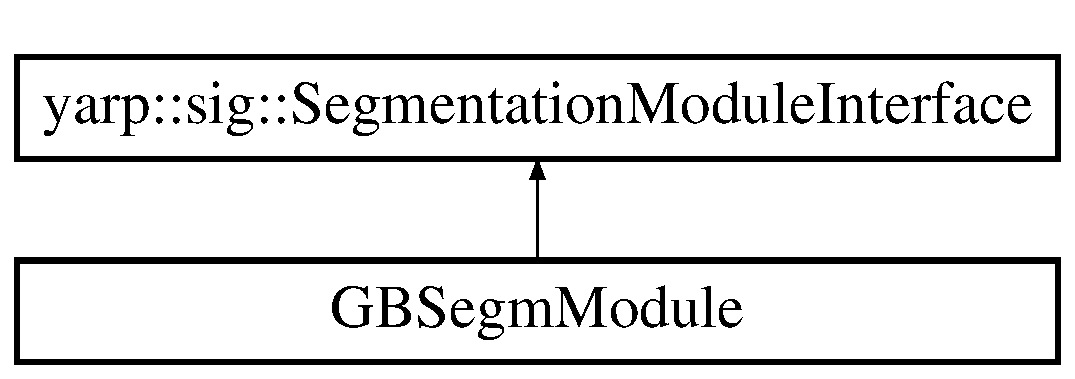
\includegraphics[height=2.000000cm]{classyarp_1_1sig_1_1SegmentationModuleInterface}
\end{center}
\end{figure}
\subsection*{Public Member Functions}
\begin{DoxyCompactItemize}
\item 
virtual void \hyperlink{classyarp_1_1sig_1_1SegmentationModuleInterface_a68f28930df5e930934c0ee56ad1f680c}{set\+\_\+sigma} (const double new\+Value)
\begin{DoxyCompactList}\small\item\em Set sigma (smoothing) parameter for the algorithm. \end{DoxyCompactList}\item 
virtual void \hyperlink{classyarp_1_1sig_1_1SegmentationModuleInterface_a2851eae0226ad68f41cd8b61d8bb1456}{set\+\_\+k} (const double new\+Value)
\begin{DoxyCompactList}\small\item\em Set k (scale factor for boundary-\/detection threshold function) parameter for the algorithm. \end{DoxyCompactList}\item 
virtual void \hyperlink{classyarp_1_1sig_1_1SegmentationModuleInterface_ad9d90ed7e362ae83e2145445a9c4301e}{set\+\_\+min\+Region} (const double new\+Value)
\begin{DoxyCompactList}\small\item\em Set min\+Region parameter for the algorithm, i.\+e., the minimum size of any segmented component. \end{DoxyCompactList}\item 
virtual double \hyperlink{classyarp_1_1sig_1_1SegmentationModuleInterface_a38431f2c63d7da8ebf20adf0ed1da4fe}{get\+\_\+sigma} ()
\begin{DoxyCompactList}\small\item\em Get sigma (smoothing) parameter for the algorithm. \end{DoxyCompactList}\item 
virtual double \hyperlink{classyarp_1_1sig_1_1SegmentationModuleInterface_a91f3d872a48599337d1d2f365ac4c31e}{get\+\_\+k} ()
\begin{DoxyCompactList}\small\item\em Get k (scale factor for boundary-\/detection threshold function) parameter for the algorithm. \end{DoxyCompactList}\item 
virtual double \hyperlink{classyarp_1_1sig_1_1SegmentationModuleInterface_a6c184aeea894f6afcc342c5aa748429d}{get\+\_\+min\+Region} ()
\begin{DoxyCompactList}\small\item\em Get min\+Region parameter for the algorithm, i.\+e., the minimum size of any segmented component. \end{DoxyCompactList}\item 
virtual int32\+\_\+t \hyperlink{classyarp_1_1sig_1_1SegmentationModuleInterface_a3c6b695fbef9e6827e7dd6b4cbbc38fe}{get\+\_\+num\+\_\+components} ()
\begin{DoxyCompactList}\small\item\em Get the number of segmented components that have been detected in the last provided image. \end{DoxyCompactList}\item 
virtual std\+::vector$<$ \hyperlink{classyarp_1_1sig_1_1Pixel}{Pixel} $>$ \hyperlink{classyarp_1_1sig_1_1SegmentationModuleInterface_a9bf0b95fbab216b2284122b0b8a36820}{get\+\_\+component\+\_\+around} (const \hyperlink{classyarp_1_1sig_1_1Pixel}{Pixel} \&obj\+Center)
\begin{DoxyCompactList}\small\item\em Get the list of pixels corresponding to the component to which a given pixel belongs. \end{DoxyCompactList}\item 
\mbox{\label{classyarp_1_1sig_1_1SegmentationModuleInterface_a8ed15458e768ad8dcc58b622a6f1d282}} 
virtual bool {\bfseries read} (yarp\+::os\+::\+Connection\+Reader \&connection) Y\+A\+R\+P\+\_\+\+O\+V\+E\+R\+R\+I\+DE
\item 
\mbox{\label{classyarp_1_1sig_1_1SegmentationModuleInterface_a14ea1dff9efc91a5099633740b3e45f9}} 
virtual std\+::vector$<$ std\+::string $>$ {\bfseries help} (const std\+::string \&function\+Name=\char`\"{}-\/-\/all\char`\"{})
\end{DoxyCompactItemize}


\subsection{Detailed Description}
Interface for module that performs graph-\/based segmentation. 

Definition at line 21 of file Segmentation\+Module\+Interface.\+h.



\subsection{Member Function Documentation}
\mbox{\label{classyarp_1_1sig_1_1SegmentationModuleInterface_a9bf0b95fbab216b2284122b0b8a36820}} 
\index{yarp\+::sig\+::\+Segmentation\+Module\+Interface@{yarp\+::sig\+::\+Segmentation\+Module\+Interface}!get\+\_\+component\+\_\+around@{get\+\_\+component\+\_\+around}}
\index{get\+\_\+component\+\_\+around@{get\+\_\+component\+\_\+around}!yarp\+::sig\+::\+Segmentation\+Module\+Interface@{yarp\+::sig\+::\+Segmentation\+Module\+Interface}}
\subsubsection{\texorpdfstring{get\+\_\+component\+\_\+around()}{get\_component\_around()}}
{\footnotesize\ttfamily std\+::vector$<$ \hyperlink{classyarp_1_1sig_1_1Pixel}{Pixel} $>$ yarp\+::sig\+::\+Segmentation\+Module\+Interface\+::get\+\_\+component\+\_\+around (\begin{DoxyParamCaption}\item[{const \hyperlink{classyarp_1_1sig_1_1Pixel}{Pixel} \&}]{obj\+Center }\end{DoxyParamCaption})\hspace{0.3cm}{\ttfamily [virtual]}}



Get the list of pixels corresponding to the component to which a given pixel belongs. 


\begin{DoxyParams}{Parameters}
{\em obj\+Center} & a pixel belonging to the region of interest \\
\hline
\end{DoxyParams}
\begin{DoxyReturn}{Returns}
list of pixels belonging to the same component as the input pixels 
\end{DoxyReturn}


Reimplemented in \hyperlink{classGBSegmModule_a0b63c53513e67c4f126e29cf7f28ad53}{G\+B\+Segm\+Module}.



Definition at line 314 of file Segmentation\+Module\+Interface.\+cpp.


\begin{DoxyCode}
314                                                                                           \{
315   std::vector<Pixel>  \_return;
316   SegmentationModuleInterface\_get\_component\_around helper;
317   helper.init(objCenter);
318   \textcolor{keywordflow}{if} (!yarp().canWrite()) \{
319     yError(\textcolor{stringliteral}{"Missing server method '%s'?"},\textcolor{stringliteral}{"std::vector<Pixel> 
       SegmentationModuleInterface::get\_component\_around(const Pixel& objCenter)"});
320   \}
321   \textcolor{keywordtype}{bool} ok = yarp().write(helper,helper);
322   \textcolor{keywordflow}{return} ok?helper.\_return:\_return;
323 \}
\end{DoxyCode}
\mbox{\label{classyarp_1_1sig_1_1SegmentationModuleInterface_a91f3d872a48599337d1d2f365ac4c31e}} 
\index{yarp\+::sig\+::\+Segmentation\+Module\+Interface@{yarp\+::sig\+::\+Segmentation\+Module\+Interface}!get\+\_\+k@{get\+\_\+k}}
\index{get\+\_\+k@{get\+\_\+k}!yarp\+::sig\+::\+Segmentation\+Module\+Interface@{yarp\+::sig\+::\+Segmentation\+Module\+Interface}}
\subsubsection{\texorpdfstring{get\+\_\+k()}{get\_k()}}
{\footnotesize\ttfamily double yarp\+::sig\+::\+Segmentation\+Module\+Interface\+::get\+\_\+k (\begin{DoxyParamCaption}{ }\end{DoxyParamCaption})\hspace{0.3cm}{\ttfamily [virtual]}}



Get k (scale factor for boundary-\/detection threshold function) parameter for the algorithm. 

\begin{DoxyReturn}{Returns}
current value for k parameter 
\end{DoxyReturn}


Reimplemented in \hyperlink{classGBSegmModule_a44bab99aa7a035e57a185673c040d2f6}{G\+B\+Segm\+Module}.



Definition at line 284 of file Segmentation\+Module\+Interface.\+cpp.


\begin{DoxyCode}
284                                           \{
285   \textcolor{keywordtype}{double} \_return = (double)0;
286   SegmentationModuleInterface\_get\_k helper;
287   helper.init();
288   \textcolor{keywordflow}{if} (!yarp().canWrite()) \{
289     yError(\textcolor{stringliteral}{"Missing server method '%s'?"},\textcolor{stringliteral}{"double SegmentationModuleInterface::get\_k()"});
290   \}
291   \textcolor{keywordtype}{bool} ok = yarp().write(helper,helper);
292   \textcolor{keywordflow}{return} ok?helper.\_return:\_return;
293 \}
\end{DoxyCode}
\mbox{\label{classyarp_1_1sig_1_1SegmentationModuleInterface_a6c184aeea894f6afcc342c5aa748429d}} 
\index{yarp\+::sig\+::\+Segmentation\+Module\+Interface@{yarp\+::sig\+::\+Segmentation\+Module\+Interface}!get\+\_\+min\+Region@{get\+\_\+min\+Region}}
\index{get\+\_\+min\+Region@{get\+\_\+min\+Region}!yarp\+::sig\+::\+Segmentation\+Module\+Interface@{yarp\+::sig\+::\+Segmentation\+Module\+Interface}}
\subsubsection{\texorpdfstring{get\+\_\+min\+Region()}{get\_minRegion()}}
{\footnotesize\ttfamily double yarp\+::sig\+::\+Segmentation\+Module\+Interface\+::get\+\_\+min\+Region (\begin{DoxyParamCaption}{ }\end{DoxyParamCaption})\hspace{0.3cm}{\ttfamily [virtual]}}



Get min\+Region parameter for the algorithm, i.\+e., the minimum size of any segmented component. 

\begin{DoxyReturn}{Returns}
current value for min\+Region parameter 
\end{DoxyReturn}


Reimplemented in \hyperlink{classGBSegmModule_a2378b95e60b406a119947aa86b5bb9c4}{G\+B\+Segm\+Module}.



Definition at line 294 of file Segmentation\+Module\+Interface.\+cpp.


\begin{DoxyCode}
294                                                   \{
295   \textcolor{keywordtype}{double} \_return = (double)0;
296   SegmentationModuleInterface\_get\_minRegion helper;
297   helper.init();
298   \textcolor{keywordflow}{if} (!yarp().canWrite()) \{
299     yError(\textcolor{stringliteral}{"Missing server method '%s'?"},\textcolor{stringliteral}{"double SegmentationModuleInterface::get\_minRegion()"});
300   \}
301   \textcolor{keywordtype}{bool} ok = yarp().write(helper,helper);
302   \textcolor{keywordflow}{return} ok?helper.\_return:\_return;
303 \}
\end{DoxyCode}
\mbox{\label{classyarp_1_1sig_1_1SegmentationModuleInterface_a3c6b695fbef9e6827e7dd6b4cbbc38fe}} 
\index{yarp\+::sig\+::\+Segmentation\+Module\+Interface@{yarp\+::sig\+::\+Segmentation\+Module\+Interface}!get\+\_\+num\+\_\+components@{get\+\_\+num\+\_\+components}}
\index{get\+\_\+num\+\_\+components@{get\+\_\+num\+\_\+components}!yarp\+::sig\+::\+Segmentation\+Module\+Interface@{yarp\+::sig\+::\+Segmentation\+Module\+Interface}}
\subsubsection{\texorpdfstring{get\+\_\+num\+\_\+components()}{get\_num\_components()}}
{\footnotesize\ttfamily int32\+\_\+t yarp\+::sig\+::\+Segmentation\+Module\+Interface\+::get\+\_\+num\+\_\+components (\begin{DoxyParamCaption}{ }\end{DoxyParamCaption})\hspace{0.3cm}{\ttfamily [virtual]}}



Get the number of segmented components that have been detected in the last provided image. 

\begin{DoxyReturn}{Returns}
number of segmented components 
\end{DoxyReturn}


Reimplemented in \hyperlink{classGBSegmModule_a655ee7c895eed07b07099133b9d8ce68}{G\+B\+Segm\+Module}.



Definition at line 304 of file Segmentation\+Module\+Interface.\+cpp.


\begin{DoxyCode}
304                                                         \{
305   int32\_t \_return = 0;
306   SegmentationModuleInterface\_get\_num\_components helper;
307   helper.init();
308   \textcolor{keywordflow}{if} (!yarp().canWrite()) \{
309     yError(\textcolor{stringliteral}{"Missing server method '%s'?"},\textcolor{stringliteral}{"int32\_t SegmentationModuleInterface::get\_num\_components()"});
310   \}
311   \textcolor{keywordtype}{bool} ok = yarp().write(helper,helper);
312   \textcolor{keywordflow}{return} ok?helper.\_return:\_return;
313 \}
\end{DoxyCode}
\mbox{\label{classyarp_1_1sig_1_1SegmentationModuleInterface_a38431f2c63d7da8ebf20adf0ed1da4fe}} 
\index{yarp\+::sig\+::\+Segmentation\+Module\+Interface@{yarp\+::sig\+::\+Segmentation\+Module\+Interface}!get\+\_\+sigma@{get\+\_\+sigma}}
\index{get\+\_\+sigma@{get\+\_\+sigma}!yarp\+::sig\+::\+Segmentation\+Module\+Interface@{yarp\+::sig\+::\+Segmentation\+Module\+Interface}}
\subsubsection{\texorpdfstring{get\+\_\+sigma()}{get\_sigma()}}
{\footnotesize\ttfamily double yarp\+::sig\+::\+Segmentation\+Module\+Interface\+::get\+\_\+sigma (\begin{DoxyParamCaption}{ }\end{DoxyParamCaption})\hspace{0.3cm}{\ttfamily [virtual]}}



Get sigma (smoothing) parameter for the algorithm. 

\begin{DoxyReturn}{Returns}
current value for sigma parameter 
\end{DoxyReturn}


Reimplemented in \hyperlink{classGBSegmModule_ae32ae1b1461e19c3a1b2f429c729ed03}{G\+B\+Segm\+Module}.



Definition at line 274 of file Segmentation\+Module\+Interface.\+cpp.


\begin{DoxyCode}
274                                               \{
275   \textcolor{keywordtype}{double} \_return = (double)0;
276   SegmentationModuleInterface\_get\_sigma helper;
277   helper.init();
278   \textcolor{keywordflow}{if} (!yarp().canWrite()) \{
279     yError(\textcolor{stringliteral}{"Missing server method '%s'?"},\textcolor{stringliteral}{"double SegmentationModuleInterface::get\_sigma()"});
280   \}
281   \textcolor{keywordtype}{bool} ok = yarp().write(helper,helper);
282   \textcolor{keywordflow}{return} ok?helper.\_return:\_return;
283 \}
\end{DoxyCode}
\mbox{\label{classyarp_1_1sig_1_1SegmentationModuleInterface_a2851eae0226ad68f41cd8b61d8bb1456}} 
\index{yarp\+::sig\+::\+Segmentation\+Module\+Interface@{yarp\+::sig\+::\+Segmentation\+Module\+Interface}!set\+\_\+k@{set\+\_\+k}}
\index{set\+\_\+k@{set\+\_\+k}!yarp\+::sig\+::\+Segmentation\+Module\+Interface@{yarp\+::sig\+::\+Segmentation\+Module\+Interface}}
\subsubsection{\texorpdfstring{set\+\_\+k()}{set\_k()}}
{\footnotesize\ttfamily void yarp\+::sig\+::\+Segmentation\+Module\+Interface\+::set\+\_\+k (\begin{DoxyParamCaption}\item[{const double}]{new\+Value }\end{DoxyParamCaption})\hspace{0.3cm}{\ttfamily [virtual]}}



Set k (scale factor for boundary-\/detection threshold function) parameter for the algorithm. 


\begin{DoxyParams}{Parameters}
{\em new\+Value} & new value for k parameter \\
\hline
\end{DoxyParams}


Reimplemented in \hyperlink{classGBSegmModule_a15129913273e221a46c428f697e40575}{G\+B\+Segm\+Module}.



Definition at line 258 of file Segmentation\+Module\+Interface.\+cpp.


\begin{DoxyCode}
258                                                              \{
259   SegmentationModuleInterface\_set\_k helper;
260   helper.init(newValue);
261   \textcolor{keywordflow}{if} (!yarp().canWrite()) \{
262     yError(\textcolor{stringliteral}{"Missing server method '%s'?"},\textcolor{stringliteral}{"void SegmentationModuleInterface::set\_k(const double newValue)"});
263   \}
264   yarp().write(helper,helper);
265 \}
\end{DoxyCode}
\mbox{\label{classyarp_1_1sig_1_1SegmentationModuleInterface_ad9d90ed7e362ae83e2145445a9c4301e}} 
\index{yarp\+::sig\+::\+Segmentation\+Module\+Interface@{yarp\+::sig\+::\+Segmentation\+Module\+Interface}!set\+\_\+min\+Region@{set\+\_\+min\+Region}}
\index{set\+\_\+min\+Region@{set\+\_\+min\+Region}!yarp\+::sig\+::\+Segmentation\+Module\+Interface@{yarp\+::sig\+::\+Segmentation\+Module\+Interface}}
\subsubsection{\texorpdfstring{set\+\_\+min\+Region()}{set\_minRegion()}}
{\footnotesize\ttfamily void yarp\+::sig\+::\+Segmentation\+Module\+Interface\+::set\+\_\+min\+Region (\begin{DoxyParamCaption}\item[{const double}]{new\+Value }\end{DoxyParamCaption})\hspace{0.3cm}{\ttfamily [virtual]}}



Set min\+Region parameter for the algorithm, i.\+e., the minimum size of any segmented component. 


\begin{DoxyParams}{Parameters}
{\em new\+Value} & new value for min\+Region parameter \\
\hline
\end{DoxyParams}


Reimplemented in \hyperlink{classGBSegmModule_ae1c722c9c774cbde4f6bfada3f0826ba}{G\+B\+Segm\+Module}.



Definition at line 266 of file Segmentation\+Module\+Interface.\+cpp.


\begin{DoxyCode}
266                                                                      \{
267   SegmentationModuleInterface\_set\_minRegion helper;
268   helper.init(newValue);
269   \textcolor{keywordflow}{if} (!yarp().canWrite()) \{
270     yError(\textcolor{stringliteral}{"Missing server method '%s'?"},\textcolor{stringliteral}{"void SegmentationModuleInterface::set\_minRegion(const double
       newValue)"});
271   \}
272   yarp().write(helper,helper);
273 \}
\end{DoxyCode}
\mbox{\label{classyarp_1_1sig_1_1SegmentationModuleInterface_a68f28930df5e930934c0ee56ad1f680c}} 
\index{yarp\+::sig\+::\+Segmentation\+Module\+Interface@{yarp\+::sig\+::\+Segmentation\+Module\+Interface}!set\+\_\+sigma@{set\+\_\+sigma}}
\index{set\+\_\+sigma@{set\+\_\+sigma}!yarp\+::sig\+::\+Segmentation\+Module\+Interface@{yarp\+::sig\+::\+Segmentation\+Module\+Interface}}
\subsubsection{\texorpdfstring{set\+\_\+sigma()}{set\_sigma()}}
{\footnotesize\ttfamily void yarp\+::sig\+::\+Segmentation\+Module\+Interface\+::set\+\_\+sigma (\begin{DoxyParamCaption}\item[{const double}]{new\+Value }\end{DoxyParamCaption})\hspace{0.3cm}{\ttfamily [virtual]}}



Set sigma (smoothing) parameter for the algorithm. 


\begin{DoxyParams}{Parameters}
{\em new\+Value} & new value for sigma parameter \\
\hline
\end{DoxyParams}


Reimplemented in \hyperlink{classGBSegmModule_a27ffe08d394d321d9f9441423d36ef5e}{G\+B\+Segm\+Module}.



Definition at line 250 of file Segmentation\+Module\+Interface.\+cpp.


\begin{DoxyCode}
250                                                                  \{
251   SegmentationModuleInterface\_set\_sigma helper;
252   helper.init(newValue);
253   \textcolor{keywordflow}{if} (!yarp().canWrite()) \{
254     yError(\textcolor{stringliteral}{"Missing server method '%s'?"},\textcolor{stringliteral}{"void SegmentationModuleInterface::set\_sigma(const double
       newValue)"});
255   \}
256   yarp().write(helper,helper);
257 \}
\end{DoxyCode}


The documentation for this class was generated from the following files\+:\begin{DoxyCompactItemize}
\item 
C\+:/dev/icub-\/contrib-\/iit/segmentation/graph\+Based/thrift\+G\+Bseg/include/Segmentation\+Module\+Interface.\+h\item 
C\+:/dev/icub-\/contrib-\/iit/segmentation/graph\+Based/thrift\+G\+Bseg/src/Segmentation\+Module\+Interface.\+cpp\end{DoxyCompactItemize}

%--- End generated contents ---

% Index
\backmatter
\newpage
\phantomsection
\clearemptydoublepage
\addcontentsline{toc}{chapter}{Index}
\printindex

\end{document}
